\pagebreak
\color{gray}
\chapter{MP-PIC: Multiphase Particle-in-Cell Method}
Our main goal is to simulate a fluidized bed reactor. In the \OF tutorials folder, a fluidized bed is pre-implemented with two different solvers. 
The first solver is called \DP and tracks each particle and models their collisions. 
Modeling each particle and collision requires a high computational effort.
Therefor in this chapter we will look at the \MP solver which mitigates the complexity by modeling particle interactions through the particle normal stress on the Eulerian grid.
On top of that particles can be grouped into parcels with similar characteristics, reducing computation time further. 
The first one gives a more accurate solution while the latter has a lower computational effort which is useful when the trend of the experiment is more important than the accuracy.
In this chapter, we will first look at an overview of approaches used for modeling gas-solid multiphase flows. Then we will look at one in detail, the \MP method, the governing equation and how they are solved numerically. 
This chapter is mainly based on the paper which first presented the \MP method \cite{MPPICFirst}.

\color{gray}
\section{Overview of Gas-Solid Multiphase Flow Solvers}
Our goal of this section is to look at a brief overview of different CFD approaches. 
These approaches can be roughly divided into two categories: The Euler-Euler methods and the Euler-Lagrange methods. 
The Eulerian-Eulerian methods model both the gas and the solid phase as a continuum. In the Euler-Lagrange model the gas is modeled as a continuous phase and the solid as a discrete phase.
The \MP-model is a hybrid model, constructed in a way that exploits the advantages of both the Euler-Euler method as well as the Euler-Lagrange method.


%\Todo{EE und EL erklären? Welche alles?} 

\begin{itemize}
    \item something about Euler-Euler and Euler-Lagrange
    \item OpenFoams DPMFoam is not the logical Lagrangian Disecrete Phase Model (which has no collision) but brobably DDPM-KTGF (Dense Discrete Phase Model incorporated with Kinetic Theory of Granular Flow)
\end{itemize}
\FloatBarrier
\begin{figure}[h!]
    \begin{tikzpicture}[
  sibling distance=8em,
  level distance=4em,
  every node/.style = {font=\normalsize},
  edge from parent/.style = {draw, -latex},
  level 1/.style={sibling distance=14em},
  level 2/.style={sibling distance=8em},
  highlight/.style={draw=kit-red, very thick}, opacity = 0.5%ellipse, inner sep=2pt}
  ]

\node[align = left, auto = right, near end]{Solid phase\\representation}
  child {node[align = left, auto = right, near end] {Discrete}
    child {node[align = left, auto = right, near end] {Particle Resolved\\Direct Numerical\\Simulations\\PR-DNS}}
    child {node[align = left, auto = right, near end] {Discrete Particle\\Model\\DPM}}
  }
  child {node[align = left, auto = right, near end] {Hybrid Models\\HM}
  child {node[align = left, auto = right, near end, highlight] {Multiphase-Particle-In-Cell\\MPPIC}}}
  child {node[align = left, auto = right, near end] {Continuum}
    child {node[align = left, auto = right, near end] {Two Fluid Model\\TFM}}
    child {node[align = left, auto = right, near end] {Mixture Model\\MM}}
  };
\end{tikzpicture}
\caption{\color{gray} Source: \url{https://www.mdpi.com/2227-7390/12/23/3700}}
\end{figure}
\FloatBarrier
\color{black}

%TODO: von wo aus anfangen? Euler/Euler bzw. Euler/Lagrange Modelle erklären?

\section{Governing equations}
In the \MP method, the fluid phase is modeled as through a continuum model and the particle phase using a Lagrangian model.
For the fluid phase mass and momentum equations are solved. For the particles the Liouville equation is solved for the distribution function of particle positions, velocities and sizes.
The particle properties are then mapped to an Eulerian grid and used to calculate the stress tensor. 
The stress tensor models particle collision which is used in the advanced particle positions. In this section we will look at the governing equation for both phases and at the interpolation operators which connect them and the numerical solution.

\subsection{Fluid Phase}
The fluid phase, in our case gas, is modeled through an Eulerian approach for incompressible flows.
The gas phase is governed by the conservation equations for mass
\begin{equation}
    \dfrac{\partial (\fvf \rf)}{\partial \tvar} + \nabla \cdot (\fvf \rf \uf) = 0,
\end{equation}
and momentum
\begin{equation}
    \label{eq:momEul}
    \dfrac{\partial (\fvf \rf \uf)}{\partial \tvar} + \nabla \cdot (\fvf \rf \uf \uf) = - \nabla \p -\nabla \cdot \fst - \boldsymbol{F} + \fvf \rf \g.
\end{equation}
Here $\uf$ is the fluid velocity and $\fvf$ the fluid volume fraction.
If not labeled otherwise, the gradient refers to the spatial component.
In the momentum term
%\Todo{Stimmen die Vorzeichen?}
%\Todo{Wie viel soll hier zu Herleitung EL?}
%To achieve multiphase coupling, we will later insert a source term. \Todo{Probably}. 
we have $\rf$ as the fluid density, $\p$ as fluid pressure, $\fst$ as the fluid stress tensor and $\g$ as the gravitational acceleration. $\F$ is the interphase momentum transfer, which will be discussed in the following subsection. 
For both equations we assume that we have no interphase mass transfer.
In the first versions of the \MP method the fluid stress tensor was omitted by setting it to zero
\begin{equation*}
    \fst = 0,
\end{equation*}
which is also assumed in this chapter.
In later \MP descriptions it is given by the Newtonian viscosity law
\begin{equation}
    \label{eq:fst}
    \fst = - \fv \left( \nabla \uf + ( \nabla \uf)^T \right) + \dfrac{2}{3} \fv ( \nabla \cdot \uf),
\end{equation}
see \cite{mathMPPIC}.
We also assume that we have an ideal gas, which we will use later in the implicit approximations. Therefor the pressure can be related to the fluid density by
\begin{equation}
\label{eq:gasDensReal}
    \dfrac{\p}{\rf^\gamma} = constant.
\end{equation}

\subsection{Solid Phase}

The solid phase is governed by the Liouville equation solving for the particle probability distribution function $\pd$
\begin{equation*}
        \dfrac{d}{dt} \int \int \pd d \up d \xp = 0
\end{equation*}
for which we can add damping terms on the right hand side to account for local collisions.

% The solid phase is treated as both a continuous phase as well as a discrete phase in the \MP method.
% The behavior of the particles is governed by the Liouville equation for the particle probability distribution function.
% Consider the domain $\Omega \subset\R^3$, %partial volume $\Omega_p \subset \R^3$ 
% velocity space $\Pi \subset \R^3$ and time interval $I = [0,\T], \ \T \in \R$. For the solid phase we define a particle distribution function %$\pd: \Omega \times \Pi \times \Op \times I \times \R \times \R \to \R^+, \ \pd(\xp, \up, \Op, t, \rp, \m) $
% \begin{equation}
%     \pd : \Omega \times \Pi \times I \times \R \to \R^+, \qquad (\xp, \up, \tvar, \m) \mapsto \pd (\xp , \up , \tvar, \m)  
% \end{equation}
% with $\xp$ the particle position, $\up$ the particle velocity, $\Op$ the particle volume, $\m$ the particle mass and $\rp$ the particle mass density.
% %Assuming that the particle Volume and particle density are constant, the particle distribution function quantifies the average number of particles having velocity $\up$ at $\xp$ with particle mass $\m$ at time $\tvar$.
% The particle density function gives the probable average number of particles per unit volume $\Np$ with a velocity in the interval $(\Vp, \Vp + \Delta \Vp)$ and mass in the interval $(\M, \M + \Delta \M)$ when integrating over the velocity and mass
% %\Todo{Ahhhh why is it called distribution and not density}
% \begin{equation}
%     \Np = \int_{\M}^{\M+\Delta \M} \int_{\Vp}^{\Vp + \Delta \Vp} \pd d \up d \m. 
% \end{equation} 
% For a small volume this can be approximated by
% \begin{equation}
%     \Np \approx \pd (\xp , \Vp , \tvar, \M) \cdot \Delta \boldsymbol{V_p} \cdot \Delta M.
% \end{equation}
% The solids volume fraction is then given by taking particles of all mass and velocities
% \begin{equation}
%     \label{eq:svf}
%     \pvf = \int \int \pd \dfrac{\m}{\rp} d \m d \up.
% \end{equation}
% % The particle size is given by
% % \begin{equation}
% %     N(\boldsymbol{x}_p, \boldsymbol{v}_p, \Omega_p, t, \rho_p, m_p) = \int f(\boldsymbol{x}_p, \boldsymbol{v}_p, \Omega_p, t, \rho_p, m_p) dv_p.
% % \end{equation}

% We assume that the total number of particles near $\xp$ with velocity $\up$ in any volume is conserved. Therefor we have
% \begin{equation}
% \label{eq:partConservation}
%     \dfrac{d}{dt} \int \int \pd d \up d \xp = 0.
% \end{equation}
% %By applying the Leipniz integral rule and, using that the volume over which we integrate is arbitrary, we transform the equation above into the Liouville equation.
% Using that the this hold for all volumes we can transform the equation above into the Liouville equation
\begin{align}
    \dfrac{\partial \pd}{\partial \tvar} + \dfrac{\partial}{\partial \xp} \left( \pd \dfrac{d \xp}{d \tvar} \right)+ \dfrac{\partial}{\partial \up} \left( \pd \dfrac{d \up}{d \tvar} \right) = 0 \\
    \label{eq:Liouville}
    \Leftrightarrow \dfrac{\partial \pd}{\partial \tvar} + \dfrac{\partial (\pd \up)}{\partial \xp} + \dfrac{\partial (\pd \Ap)}{\partial \up} = 0. % \left( \dfrac{\partial f}{\partial t} \right)_{coll}.
\end{align}
Here $\Ap$ is the particle acceleration. The term is defined by Newton's equations of motion. The forces acting on the particle are aerodynamic drag, pressure gradient, interparticle stress and gravity.
The equations are given by
\begin{align}
    \dfrac{d \xp}{d \tvar} &= \up, \\
    \label{eq:accel}
    \Ap = \dfrac{d \up}{d \tvar} &=\d(\uf - \up) - \dfrac{1}{\rp} \nabla_{\xp} \p - \dfrac{1}{\pvf \rp} \nabla_{\xp} \scs + \g.
\end{align}
The \MP method accounts for collisions by the spatial gradient of the solid stress. 
To model collison behavior more locally collison terms were added to the right hand side of the Liouville equation \eqref{eq:Liouville} 
\begin{equation}
    \label{eq:LiouCollide}
    \dfrac{\partial \pd}{\partial \tvar} + \dfrac{\partial (\pd \up)}{\partial \xp} + \dfrac{\partial (\pd \Ap)}{\partial \up} = \left( \dfrac{\partial \pd}{\partial 
    \tvar} \right)_{coll}.
\end{equation}
We will cover these damping terms later in this chapter, see \ref{sec:damping}.

Here \uf is the mean flow fluid velocity, $\d(\Op,\up, \xp,\tvar)$ is the drag function and $\p$ is the mean flow fluid thermodynamic pressure, $\scs(\xp, \tvar)$ is the solids contact stress.

To arrive at the interphase momentum transfer function we look at the moments from the Liouville equation \eqref{eq:Liouville}.
We multiply the equation by $\m$ and integrate over the mass and velocity. This yields a connection between the field properties and the interaction between the two phases
\begin{align*}
    \int \int \m \left( \dfrac{\partial \pd}{\partial \tvar} + \nabla_{\xp} \cdot (\pd \up) + \nabla_{\up} \cdot (\pd \Ap)\right) d \up d \m = 0 \\
    \Leftrightarrow
    \dfrac{\partial }{\partial \tvar} \int \int \pd \m d \m d \up + \nabla_x \cdot \left( \int \int m \pd \up d\up d \m \right) = 0\\
    \stackrel{\eqref{eq:svf}}{\Leftrightarrow} \dfrac{\partial (\pvf \rp )}{\partial t} + \nabla_{\xp} \cdot (\pvf \rp \overline{\up}) = 0    
\end{align*}
with the third term being zero by using integration by parts and $\pd \to 0$ for $\lvert \up \rvert \to \infty$. 
The term for the mean particle velocity is
\begin{equation*}
    \overline{\up} = \dfrac{1}{\rp \pvf}\MultiIntegral{2} \pd \m \up d\m d \up.
\end{equation*}

%In this case our particle distribution function depends only on particle position, velocity, mass and time. 
%For a particle distribution function that instead of the mass would depend on the density and volume we would need to integrate over these factors.
The term is called the particle conservation equation.
We obtain the second momentum term by multiplying the Liouville equation \eqref{eq:Liouville} by $\m \up$ and again integrating over $\m$ and \up
\begin{equation}
\label{eq:mom2Begin}
    \MultiIntegral{2} \m \up \left( \dfrac{\partial \pd}{\partial \tvar} + \nabla_{\xp} \cdot (\pd \up) + \nabla_{\up} \cdot \left(\pd
    \left(\d(\uf - \up) - \dfrac{1}{\rp} \dfrac{\partial \p}{\partial \xp} - \dfrac{1}{\pvf \rp} \dfrac{\partial \scs}{\partial \xp} + \g \right)
    \right)\right) d \up d \m = 0
\end{equation}
With partial integration and using again that $\pd \to 0$ for $\lvert \up \rvert \to \infty$ we have
\begin{equation*}
    \int \int \m \up \nabla_{\up} \cdot (\pd \Ap ) d \up d \m = - \int \int \m \Ap \pd d \up d \m.
\end{equation*}
Using the mean particle velocity to reformulate
\begin{equation*}
    \int \int \m \up \dfrac{\partial \pd}{\partial \tvar} d \up d \m = \dfrac{\partial}{\partial \tvar} (\rp \pvf \overline{\up} )
\end{equation*}
and
\begin{equation*}
    \MultiIntegral{2} \m \up \up \pd d \up d \m = \rp \overline{\up} \overline{\up} + \MultiIntegral{2} \m (\up - \overline{\up}) ( \up - \overline{\up}) \pd d \up d \m.
\end{equation*}
By replacing the corresponding terms in equation \eqref{eq:mom2Begin} and multiplying by $\pvf \rp$ we then have the particle momentum equation
\begin{equation}
    \begin{aligned}
\label{eq:secondMomentum}
    %\MultiIntegral{2} \m \up \left( \dfrac{\partial \pd}{\partial \tvar} \right. & \left.+ \nabla_{\xp} \cdot (\pd \up) + \nabla_{\up} \cdot \left(\pd
    %\left(\d(\uf - \up) - \dfrac{1}{\rp} \dfrac{\partial \p}{\partial \xp} - \dfrac{1}{\pvf \rp} \dfrac{\partial \scs}{\partial \xp} + \g \right)
    %\right)\right) d \up d \m = 0 \\
    %\Leftrightarrow 
    \dfrac{\partial ( \pvf \rp \overline{\up})}{\partial t} &+ \nabla_{\xp} \cdot (\pvf \rp \overline{\up} \overline{\up} ) + \nabla \scs + \pvf \nabla \p \\ &= \pvf \rp \g + \MultiIntegral{2} \pd \m \d (\uf - \up) d \m d\up - \nabla \cdot \left[ \MultiIntegral{2} \pd \m (\up - \overline{\up}) (\up - \overline{\up}) d \m d \up \right].
    \end{aligned}
\end{equation}
The last term in the equation mimics the kinematic stress from the particle velocity fluctuations, similar to Reynold stress. The fourth and sixth term depend on both phases and therefor contribute to the interphase momentum transfer function, which models the particle force per unit volume on the fluid phase
%\Todo{Second momentum term}
\begin{equation}
    \label{eq:InterMomTrans}
    \F = \int \int \pd \m [\d (\uf - \up) - \dfrac{1}{\rp} \nabla \p] d\m d\up.
\end{equation}
We can split the integral up into two terms. The first represents the momentum exchange due to aerodynamic drag.
For more detailed models we can use particle density and volume instead of mass.
Often in the gas momentum equation \eqref{eq:momEul} the pressure gradient is multiplied by the gas volume fraction. Taking the second term in the equation above \eqref{eq:InterMomTrans} we receive this term by the following calculation.
We know that for the volume fraction
\begin{equation}
    \fvf + \pvf = 1 \qquad \nabla p - \fvf \nabla p = \pvf \nabla p
\end{equation}
holds.
From equation \eqref{eq:svf} we have
\begin{equation}
    \fvf \nabla p =  \int \int \pd \m \dfrac{1}{\rp} \nabla \p d\m d\up
\end{equation}
which is included in equation \eqref{eq:InterMomTrans} in the interface momentum transfer function. 
By setting both terms against one another only $\pvf \nabla p$ remains in the equation \eqref{eq:InterMomTrans}.

% In later versions, the \MP method was extended to two-dimensional problems and a scheme for three-dimensional models was introduced. 
% On top of that a collision term was added on the right hand side of the Liouville equation. 
% The collision operator in general reads


In a later paper (\cite{MPInterpolation}) the \MP method was also extended to two-dimensional problems and a scheme for three-dimensional models was introduced. 
A second term  was introduced later (\cite{damp}, \cite{isotropy})  which represents the scattering from particle collisions and is called return-to-isotropy.
These terms improve upon the \MP method by modeling particle collisions locally as opposed to spatial gradients of the particle gradient.
The terms will be explained in the following.
\begin{equation}
    \left( \frac{\partial \pd}{\partial \tvar} \right)_{coll} = \underbrace{\dfrac{\pdd - \pd}{\sd}}_{\text{daming term}} + \underbrace{\dfrac{\pdi - \pd}{\si}}_{\text{return-to-isotropy}}.
\end{equation}

\color{gray}
\subsubsection{Damping term}
\label{sec:damping}
The damping term above is the BGK-collision term with \sd \ as the collision damping time and \pdd \ as
\begin{equation}
    \label{eq:colDamp}
    \pdd = \left[ \int \pd d \up \right] \delta (\up - \nup).
\end{equation}
with the mass-averaged velocity
\begin{equation}
    \nup = \dfrac{\MultiIntegral{2}  \pd \m \up d \m d  \up}{\MultiIntegral{2} \pd \m d \m d \up}
\end{equation}
\Todo{$\up$ mess fixen}
%\Todo{BGK Term genau erklären?}
It was introduced by Bhatnagar, Gross and Krook and is used frequently in lattice Boltzmann methods.
Therefor the particle velocities are distributed symmetrically around the local mass-averaged particle velocity \nup. This is due to collisions tending to relax the distribution function to the equilibrium \pdd.

In %TODO add ref
it is shown that the equation \eqref{eq:colDamp} is equal to the one with more dependencies.


For a constant relaxation time $\sd$ the analytical solution to the damping term is given by
\begin{equation}
    \label{eq:BGKanalytical}
    \pd = e^{-\frac{\tvar}{\sd}} \pd^n + \left(1-e^{- \frac{t}{\sd}} \right) \pd_{D}.
\end{equation}
which we can quickly verify by partially deriving the equation above
\begin{equation}
    \dfrac{\partial \pd}{\partial \tvar} = - \dfrac{1}{\sd} e^{- \frac{t}{\sd}} \pd_n + \dfrac{1}{\sd} e^{- \frac{t}{\sd}} \pd_D = \dfrac{\pd_D - \pd}{\sd}.
\end{equation}

The damping time is discussed in the section numerical discretizations.


\subsubsection{Return-to-Isotropy}

\color{black}
\section{Numerical implementation and discretizations}
\subsection{Parcel Grouping}
\Todo{Bisschen Überleitung einfügen}
To reduce computing time for a large number of particles the \MP method can group particles with similar characteristics. The number of particles in a parcel is given by the statistical weight of the parcel \wp.
The parcels each contain \wp \ particles with identical particle mass $\m$, velocity $\up$ and position $\xp$. 
The sketch below illustrates the grouping of particles. The sketches on the left and in the middle are for illustration purposes only. In the \MP method the particles are represented through point masses, infinitesimal small points and the properties with properties assigned to them.
\FloatBarrier
\begin{figure}[h!]
\centering
\begin{tikzpicture}

% Define colors
\definecolor{purple}{RGB}{153, 51, 255}
\definecolor{cyan}{RGB}{0, 204, 255}
\definecolor{orange}{RGB}{255, 153, 51}
\definecolor{darkpurple}{RGB}{102, 0, 153}

% Function to draw a frame
\newcommand{\frameaxes}[3]{
  \draw[thick] (#1,#2) circle (#3);
  \draw[-{Latex[length=1.2mm]}] (#1,#2) -- ++(0,0.2);
  \draw[-{Latex[length=1.2mm]}] (#1,#2) -- ++(0.2,0);
}

% Draw left clusters
% Orange group
\draw[orange, dotted, thick] plot [smooth cycle, tension=0.8] coordinates {(-4.2,-2.0) (-2.8,-2.8) (-2.4,-2.2) (-2.8, -1.9) (-3.1,-1.0)};
\frameaxes{-3.7}{-2.0}{0.2}
\frameaxes{-3.3}{-1.5}{0.2}
\frameaxes{-3.0}{-2.4}{0.2}

% Cyan group
\draw[cyan, dotted, thick] plot [smooth cycle, tension=0.8] coordinates {(-2.3,1.5) (-0.1,-0.2) (-2.2,-2.0) (-2.7,-0.5)};
\frameaxes{-2.0}{0.7}{0.6}
\frameaxes{-1.0}{-0.2}{0.6}
\frameaxes{-2.0}{-1.1}{0.6}

% Purple group
\draw[darkpurple, dotted, thick] plot [smooth cycle, tension=0.8] coordinates {(-4.6,1) (-3.3,2.3) (-2.4, 2.1) (-3.0,1.1) (-3.1,-0.4)};
\frameaxes{-4.0}{1.3}{0.3}
\frameaxes{-3.0}{2}{0.3}
\frameaxes{-3.4}{0.2}{0.3}

% Central dashed line
\draw[black, thick, dashed] (0,-3) -- (0,2.5);

% Right-side isolated frames and arrows
% Purple arrow + frame
%\draw[purple, ->, dotted, thick] (-2.5,1.8) .. controls (0.5,2.2) .. (1.1,1.6);
\draw[thick, color=purple] (1.5,1.2) circle (0.52);
\draw[-{Latex[length=1.2mm]}] (1.5,1.2) -- ++(0,0.2);
\draw[-{Latex[length=1.2mm]}] (1.5,1.2) -- ++(0.2,0);


% Cyan arrow + frame
%\draw[cyan, ->, dotted, thick] (-0.1,0.1) .. controls (1,-0.5) .. (2.6,-0.1);
\draw[thick, color=cyan] (3.5,0.5) circle (1.04);
\draw[-{Latex[length=1.2mm]}] (3.5,0.5) -- ++(0,0.2);
\draw[-{Latex[length=1.2mm]}] (3.5,0.5) -- ++(0.2,0);

% Orange arrow + frame
%\draw[orange, ->, dotted, thick] (-2.4,-2.3) .. controls (0,-3) .. (1.5,-2.1);
\draw[thick, color=orange] (1.8,-1.8) circle (0.35);
\draw[-{Latex[length=1.2mm]}] (1.8,-1.8) -- ++(0,0.2);
\draw[-{Latex[length=1.2mm]}] (1.8,-1.8) -- ++(0.2,0);

\draw[black, thick, dashed] (5,-3) -- (5,2.5);

\filldraw[color=cyan, fill, very thick](8.5,0.5) circle (0.1);
\filldraw[color=purple, fill, very thick](6.5,1.25) circle (0.1);
\filldraw[color=orange, fill, very thick](6.8,-1.8) circle (0.1);
\draw[-{Latex[length=1.2mm]}] (6.8,-1.8) -- ++(0,0.2);
\draw[-{Latex[length=1.2mm]}] (6.8,-1.8) -- ++(0.2,0);
\draw[-{Latex[length=1.2mm]}] (6.5,1.25) -- ++(0,0.2);
\draw[-{Latex[length=1.2mm]}] (6.5,1.25) -- ++(0.2,0);
\draw[-{Latex[length=1.2mm]}] (8.5,0.5) -- ++(0,0.2);
\draw[-{Latex[length=1.2mm]}] (8.5,0.5) -- ++(0.2,0);
\end{tikzpicture}
\caption{Grouping particles on the left to parcels on the right with $\wp = 3$. On the right particles as "point mass" as used in the Lagragian framework. The two sketches on the left are for illustrational purposes for how grouping works and do not represent the particles used for calculation.}
\end{figure}
\FloatBarrier


\subsection{Interpolation Operators}
In the \MP method the solid phase is partially treated as a continuous phase to reduce computing time.
Different properties of the solid phase, for example the volume fraction $\pvf$ are mapped to and from the Eulerian grid.
The interpolation operators, which are defined for one dimension in \cite{MPPICFirst} were extended first to two dimensions \cite{MP2d} and then to three dimensions in \cite{MPInterpolation}.
The \MP method uses a staggered gird with momentum properties, for example velocity, interpolated from the cell faces to the particles while scalar properties, like the volume fraction are interpolated from the cell centers.
For a particle located at $\xp$ we define an interpolation operator for the cell center for the $x$-component $\xpx$ as
\begin{equation}
    \ip_i^\x (\xp) = \begin{cases}
        0 & \x_{i-1} \geq \xpx, \ \xpx \geq \x_{i+1} \\
        1 & \xpx = \x_{i}.
    \end{cases}
\end{equation}
The interpolation operator for the $x$-coordinate is independent of the $y$ and $z$ coordinate.
For this section we use a linear interpolation operator
\begin{equation}
    \ip_{i}^\x = \dfrac{\x_{i+1}- \xpx}{\x_{i+1} - \x_i} \quad \x_{i} < \xpx < \x_{i+1}
\end{equation}
which can be seen in the following figure, but other interpolation schemes are also applicable.
In one dimension the the interpolation is only supported by two cell centers while in two dimensions we use the four surrounding nodes. 


\begin{figure}[h!]
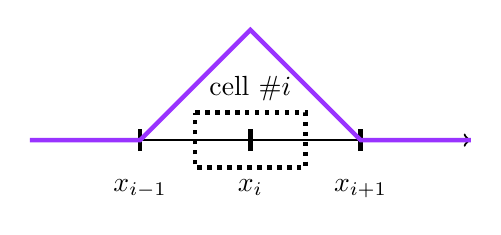
\begin{tikzpicture}[ultra thick, scale = 1.4]
    \draw[->,thick] (0,0) -- (4,0);
    \draw (1, -0.1) -- (1 , 0.1);
    \draw (2, -0.1) -- (2 , 0.1);
    \draw (3, -0.1) -- (3 , 0.1);
    \draw[purple] (0,0) -- (1,0) -- (2,1) -- (3,0) -- (4,0);
    \node[anchor = north] at (1,-0.25) {$x_{i-1}$};
    \node[anchor = north] at (2,-0.25) {$x_{i}$};
    \node[anchor = north] at (3,-0.25) {$x_{i+1}$};
    \draw[dotted] (1.5, 0.25) -- (2.5,0.25) -- (2.5, -0.25) -- (1.5, -0.25) -- cycle;
    \node[anchor = south] at (2, 0.25) {cell $\# i$};
\end{tikzpicture}
\hfill
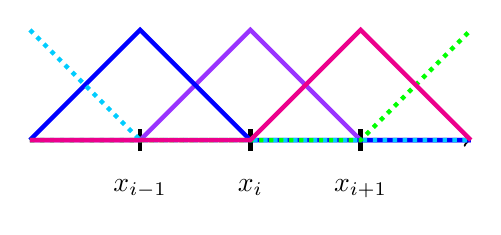
\begin{tikzpicture}[ultra thick, scale = 1.4]
    \draw[->,thick] (0,0) -- (4,0);
    \draw (1, -0.1) -- (1 , 0.1);
    \draw (2, -0.1) -- (2 , 0.1);
    \draw (3, -0.1) -- (3 , 0.1);
    \draw[purple] (0,0) -- (1,0) -- (2,1) -- (3,0) -- (4,0);
    \draw[blue] (0,0) -- (1,1) -- (2,0) -- (4,0);
    \draw[cyan, dotted] (0,1) -- (1,0) -- (4,0);
    \draw[green, dotted] (0,0) -- (3,0) -- (4,1);
    \draw[magenta] (0,0) -- (2,0) -- (3,1) -- (4,0);
    \node[anchor = north] at (1,-0.25) {$x_{i-1}$};
    \node[anchor = north] at (2,-0.25) {$x_{i}$};
    \node[anchor = north] at (3,-0.25) {$x_{i+1}$};
    %\draw[dotted] (1.5, 0.25) -- (2.5,0.25) -- (2.5, -0.25) -- (1.5, -0.25) -- cycle;
    %\node[anchor = south] at (2, 0.25) {cell $\# i$};
\end{tikzpicture}
\caption{Linear interpolation operator. On the right $\ip_i$ on the right $\ip_{i-1}$, $\ip_{i}$, $\ip_{i+1}$.}
\end{figure}

%\Todo{Add 2d}
\begin{figure}
\label{fig:int2D}
\tdplotsetmaincoords{70}{120}
    \begin{tikzpicture}[tdplot_main_coords,line cap=butt,line join=round,c/.style={circle,fill,inner sep=1.25pt},
        declare function={a=4;h=3;}]
   % Outer square corners
  \coordinate (Z) at (-a/4, -a/4, 0);
  \coordinate (Y) at (5*a/4, -a/4, 0);
  \coordinate (X) at (5*a/4, 5*a/4, 0);
  \coordinate (W) at (-a/4, 5*a/4, 0);
  \coordinate (V) at (-a/4, a/2 ,0);
  \coordinate (U) at (a/2, 5*a/4,0);
  \coordinate (T) at (a/2, -a/4,0);
  \coordinate (R) at (5*a/4, a/2,0);

  % Outer square
  \draw[dotted] (Z) -- (Y) -- (X) -- (W) -- cycle;

  % Grid of 16 squares (4x4)
  \foreach \i in {0,1,2} {
    \foreach \j in {0,1,2} {
      %\draw[dotted](-a/4 + \i*a/2, -a/4 + \j*a/2, 0) rectangle         (-a/4 + (\i+1)*a/2, -a/4 + (\j+1)*a/2, 0);
      \pgfmathsetmacro{\xlow}{-a/4 + \i*a/2}
    \pgfmathsetmacro{\ylow}{-a/4 + \j*a/2}
    \pgfmathsetmacro{\xhigh}{-a/4 + (\i+1)*a/2}
    \pgfmathsetmacro{\yhigh}{-a/4 + (\j+1)*a/2}
    \draw[dotted] (\xlow,\ylow,0) -- (\xlow,\yhigh,0) -- (\xhigh,\yhigh,0) -- (\xhigh,\ylow,0) --cycle;
    }
  }
        \path
        (0,0,0) coordinate (A)
        (a,0,0) coordinate (B)
        (a,a,0) coordinate (C)
        (0,a,0) coordinate (D)
        (0,a/2,0) coordinate (E)
        (a/2,0,0) coordinate (F)
        (a,a/2,0) coordinate (G)
        (a/2,a,0) coordinate (H)
    (a/2,a/2,0) coordinate (O)      
    (a/2,a/2,h)  coordinate (S);
\shade[shading=axis, bottom color=purple!60, top color=black!80, opacity =0.5] (S) -- (A) -- (B) -- cycle;
\shade[shading=axis, bottom color=purple!60, top color=black!80, opacity =0.5] (S) -- (A) -- (D) -- cycle;
\shade[shading=axis, bottom color=purple!60, top color=black!80, opacity =0.5] (S) -- (C) -- (D) -- cycle;
\shade[shading=axis, bottom color=purple!60, top color=black!80, opacity =0.5] (S) -- (C) -- (B) -- cycle;
\shade[shading=axis, right color=purple!60, left color=purple!60, opacity=0.5]
  (Y) -- (Z) -- (A) -- (B) -- cycle;
\shade[shading=axis, bottom color=purple!60, top color=purple!60, shading angle=90, opacity=0.5] 
  (Y) -- (X) -- (C) -- (B) -- cycle;
\shade[shading=axis, top color=purple!60, bottom color=purple!60, opacity =0.5] (X) -- (W) -- (D) -- (C) -- cycle;
\shade[shading=axis, top color=purple!60, bottom color=purple!60, opacity =0.5] (W) -- (Z) -- (A) -- (D) -- cycle;
%\draw (S) -- (D) -- (C) -- (B) -- cycle (S) -- (C);
\draw[purple,thick] (S) -- (D);
\draw[purple,thick] (S) -- (C);
\draw[purple,thick] (S) -- (B);
\draw[purple,thick] (S) -- (G);
\draw[purple,thick] (S) -- (H);
\draw[purple,thick] (C) -- (X);
\draw[purple,thick] (A) -- (Z);
\draw[purple,thick] (B) -- (Y);
\draw[purple,thick] (D) -- (W);
%RTUV
\draw[purple,thick] (F) -- (T);
\draw[purple,thick] (E) -- (V);
\draw[purple,thick] (G) -- (R);
\draw[purple,thick] (H) -- (U);
%\draw[dashed] (S) -- (A) --(D) (A) -- (B) (S);
\draw[purple,thick,dashed] (S) -- (E);
\draw[purple, thick, dashed] (S) -- (F);
\draw[purple,dashed,thick] (S) -- (A);


        \path foreach \p/\g/\lbl in {A/-50/x_{i-1,j-1},B/-90/x_{i-1,j+1},C/-90/x_{i+1,j+1},D/-50/x_{i+1,j-1},S/0/1,O/180/x_{i,j},E/-90/x_{i,j-1},F/-90/x_{i-1,j},G/-90/x_{i,j+1},H/-90/x_{i+1,j}}{(\p)node[c]{}+(\g:4mm) node{$\lbl$}};  
    \end{tikzpicture}
    \hfill
    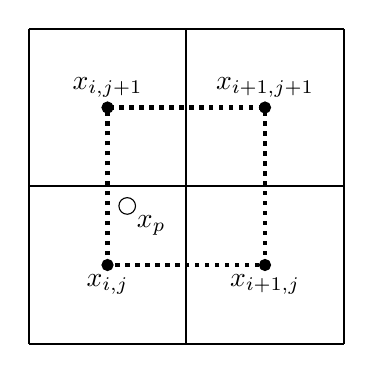
\begin{tikzpicture}[declare function={a=2;}]
        \coordinate (A) at (0,0);
        \coordinate (B) at (a,0);
        \coordinate (C) at (2*a,0);
        \coordinate (D) at (0,a);
        \coordinate (E) at (a,a);
        \coordinate (F) at (2*a,a);
        \coordinate (G) at (0,2*a);
        \coordinate (H) at (a,2*a);
        \coordinate (I) at (2*a,2*a);
        \draw[thick] (A) -- (C);
        \draw[thick] (D) -- (F);
        \draw[thick] (G) -- (I);        
        \draw[thick] (A) -- (G);
        \draw[thick] (B) -- (H);
        \draw[thick] (C) -- (I);     
        \filldraw[black] (a/2,a/2) circle (2pt) node[anchor = north]{$x_{i,j}$};
        \filldraw[black] (3*a/2,a/2) circle (2pt) node[anchor = north]{$x_{i+1,j}$};
        \filldraw[black] (a/2,3*a/2) circle (2pt) node[anchor = south]{$x_{i,j+1}$};
        \filldraw[black] (3*a/2,3*a/2) circle (2pt) node[anchor = south]{$x_{i+1,j+1}$};
        \draw (5*a/8,7*a/8) circle (3pt) node[anchor = north west]{$x_p$};
        \draw[dotted,ultra thick] (a/2,a/2) -- (a/2,3*a/2) -- (3*a/2, 3*a/2) -- (3*a/2, a/2) -- cycle;
        %\node at (a/2,a/2) {$x_{i,j}$};
    \end{tikzpicture}
    \caption{Interpolation in two dimensions. On the right all cell centers used for the interpolation of the particle, on the left a linear interpolation function for the cell center $i,j$.}
\end{figure}


% \begin{figure}[h!]
%     \begin{tikzpicture}[scale = 0.4, font = \huge]
%         \begin{axis}[
%     axis lines=left,
%     xmin=-3, xmax=3,
%     ymin=0, ymax=1,
%     domain=-3:3,
%     samples=200,
%     width=18cm,
%     height=6cm,
%     axis line style={->},
%     xtick = {-2,-1,0,1,2},
%     xticklabels={$x_{i-2}$, $x_{i-1}$,$x_i$,$x_{i+1}$,$x_{i+2}$},
%     ytick={1.0}
%     ]
%     \addplot[red, ultra thick] (-3,0) -- (-1,0) -- (0,1) -- (1,0) -- (3,0);
%     \addplot[red, ultra thick, domain=-3:-1] {0};
%     \addplot[red, ultra thick, domain=-1:0] {1-abs(x)/(1)};
%     \addplot[red, ultra thick, domain=0:1] {1-abs(x)/(1)};
%     \addplot[red, ultra thick, domain=1:3] {0};
%     \end{axis}
%     \end{tikzpicture}
%     \caption{Linear interpolation for the cell centers}
% \end{figure}
% The \MP-method uses the interpolation operator both for cell faces and for cell center interpolation.
% For cell faces the interpolation operators are shifted by half a cell.
% \begin{equation*}
%     \ifg_{i+1/2}^\x (\x_p) = \begin{cases}
%         0 & \x_{i-1/2} \geq \x_p \geq \x_{i+1/2} \\
%         1 & \x_p = \x_{i+1/2}
%     \end{cases}
% \end{equation*}
The interpolation operator satisfies
\begin{equation*}
    \sum_{\xi} \ip_\xi^\x (\x_p) =1
\end{equation*}
when summing over all Eulerian cells this holds for $\ip$.
For the linear case this can be observed in the sketch above.

In the two dimensional case the grid properties are mapped to the particle by using the four enclosing cell centers, see figure \ref{fig:2dintall}. 
Interpolating a quantity $Q$ from the Eulerian grid to the particle position we use
\begin{equation*}
    Q_p = \ip_{i,j} (\xp) Q_{i,j} + \ip_{i+1,j} (\xp) Q_{i+1,j}+ \ip_{i,j+1} (\xp) Q_{i,j+1}+ \ip_{i+1,j+1} (\xp) Q_{i+1,j+1}
\end{equation*}
with the two dimensional interpolation operator being formed by the product of the two one dimensional operators
\begin{equation*}
    \ip_{i,j} = \ip_i^\x \ip_j^y.
\end{equation*}


Analogously, in three dimensions we have
\begin{equation*}
    \ip_{i,j,k} = \ip^x_i \ip^y_j \ip^z_k,
\end{equation*}
with the operators $\ip^y$ and $\ip^z$ analogue to $\ip^z$ and the interpolation of grid quantities is
\begin{equation*}
    \gp_p = \ip_\xi ( \xp) \gp_\xi.
\end{equation*}

For example the discrete particle volume fraction is defined via the interpolation
\begin{equation*}
    \pvf_{p_{i,j,k}} = \dfrac{1}{\gcv_{i,j,k}} \sum_{\kappa = 1}^{\Np} \wp \gcv_{p_{i,j,k}} \ip_{i,j,k} (\x_{p_\kappa}).
\end{equation*}
The product of interpolation operators for a grid property $\gp$ where the property is mapped to a particle location and the to the grid is defined as
\begin{equation*}
    \ip_\zeta (\xp) \sum_{\xi}^8 \ip_\xi (\xp) \gp_\xi = \sum_{\xi}^{8} \ip_\zeta.
\end{equation*}
The product of two interpolation operators for cells is defined as
\begin{equation}
\label{eq:ipOrtho}
    \ip_\zeta(\boldsymbol{\x}_{p_{\kappa}})\ip_{\xi} (\boldsymbol{x}_{p_\iota}) = \begin{cases}
        \ip_{\xi}(\boldsymbol{x}_{p_\kappa}) & \text{if } \xi = \zeta \text{ and } \iota = \kappa \\
        0 & \text{else}.
    \end{cases}
\end{equation} 

% as well as the gradient
% \begin{equation*}
%     \nabla \gp_p = \sum_{\xi =1}^{N} \nabla \ip_\xi (\xp) \gp_\xi + \sum_{\xi =1}^{N} \ip_\xi ( \xp) (\nabla \gp)_{\xi}.
% \end{equation*}
For the one dimensional case we can calculate the spatial derivative of the linear interpolation operator with the help of the cell-face interpolation function. For an equidistant grid this is
\begin{equation*}
    \ifg_{i+1/2} = \begin{cases}
        1 & \text{if }   \x_i \leq \x_p < \x_{i+1} \\
        0 & \text{if }   \x_p < \x_{i} \text{ or } \x \geq \x_{i+1}.
    \end{cases} \qquad \hspace{1cm}
    \label{eq:gradInterp}
    \dfrac{\partial \ip_i}{\partial \x} = \dfrac{1}{\Delta \x} ( \ifg_{i-1/2} - \ifg_{i+1/2})
\end{equation*}
\begin{figure}
    \centering
    \begin{subfigure}[b]{0.45 \linewidth}
    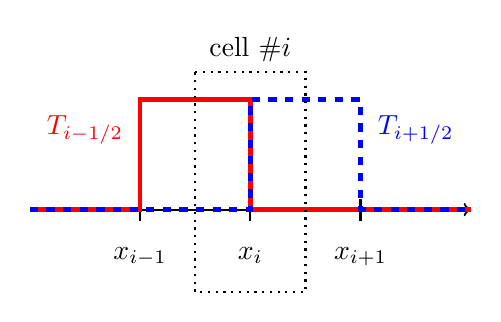
\begin{tikzpicture}[thick, scale = 1.4]
    \draw[->] (0,0) -- (4,0);
    \draw (1, -0.1) -- (1 , 0.1);
    \draw (2, -0.1) -- (2 , 0.1);
    \draw (3, -0.1) -- (3 , 0.1);
    \draw[red,ultra thick] (0,0) -- (1,0) -- (1,1) -- (2,1) -- (2,0) -- (4,0);
    \draw[blue,ultra thick,dashed] (0,0) -- (2,0) -- (2,1) -- (3,1) -- (3,0) -- (4,0);
    \node[anchor = north] at (1,-0.25) {$x_{i-1}$};
    \node[anchor = north] at (2,-0.25) {$x_{i}$};
    \node[anchor = north] at (3,-0.25) {$x_{i+1}$};
    \draw[dotted] (1.5, 1.25) -- (2.5,1.25) -- (2.5, -0.75) -- (1.5, -0.75) -- cycle;
    \node[anchor = south,red] at (0.5, 0.5) {$T_{i-1/2}$};
    \node[anchor = south,blue] at (3.5,0.5) {$T_{i+1/2}$};
    \node[anchor = south] at (2, 1.25) {cell $\# i$};
\end{tikzpicture}
    \label{fig:placeholder}
    \caption{Top hat function for the the cell faces $i-\frac{1}{2}$ (red) and $i+\frac{1}{2}$ (blue).}
    \end{subfigure}
    \hfill
    \begin{subfigure}[b]{0.45 \linewidth}
    \centering
    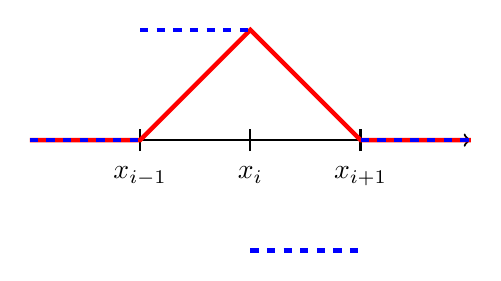
\begin{tikzpicture}[thick, scale = 1.4]
    \draw[->] (0,0) -- (4,0);
    \draw (1, -0.1) -- (1 , 0.1);
    \draw (2, -0.1) -- (2 , 0.1);
    \draw (3, -0.1) -- (3 , 0.1);
    \draw[red, ultra thick] (0,0) -- (1,0) -- (2,1) -- (3,0) -- (4,0);
    \draw[blue,dashed,ultra thick] (0,0) -- (1,0);
    \draw[blue,dashed, ultra thick] (1,1) -- (2,1);
    \draw[blue,dashed, ultra thick](2,-1) -- (3,-1);
    \draw[blue, dashed, ultra thick] (3,0) -- (4,0);
    \node[anchor = north] at (1,-0.15) {$x_{i-1}$};
    \node[anchor = north] at (2,-0.15) {$x_{i}$};
    \node[anchor = north] at (3,-0.15) {$x_{i+1}$};
    %\draw[dotted] (1.5, 0.25) -- (2.5,0.25) -- (2.5, -0.25) -- (1.5, -0.25) -- cycle;
    %\node[anchor = south] at (2, 0.25) {cell $\# i$};
\end{tikzpicture}
\caption{Interpolation operator $\ip_i$ in purple and its gradient in blue. For illustration purposes the grid has a spacing of $\Delta x = 1$.}
\end{subfigure}
\caption{Top hat function and linear interpolation with gradient.}
\end{figure}

In two dimensions we need to choose the cell faces we want to use for the interpolation. In figure \ref{fig:2dintall} we can see the velocities at the cell face centers which we will use in the following. 

\begin{figure}[htbp]
    \centering
    \begin{subfigure}[t]{0.4\textwidth}
    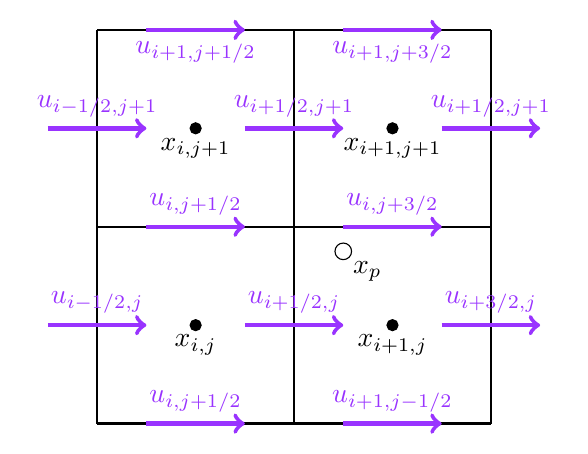
\begin{tikzpicture}[declare function={a=2.5;}]
        \coordinate (A) at (0,0);
        \coordinate (B) at (a,0);
        \coordinate (C) at (2*a,0);
        \coordinate (D) at (0,a);
        \coordinate (E) at (a,a);
        \coordinate (F) at (2*a,a);
        \coordinate (G) at (0,2*a);
        \coordinate (H) at (a,2*a);
        \coordinate (I) at (2*a,2*a);
        \draw[thick] (A) -- (C);
        \draw[thick] (D) -- (F);
        \draw[thick] (G) -- (I);        
        \draw[thick] (A) -- (G);
        \draw[thick] (B) -- (H);
        \draw[thick] (C) -- (I);     
        \filldraw[black] (a/2,a/2) circle (2pt) node[anchor = north]{$x_{i,j}$};
        \filldraw[black] (3*a/2,a/2) circle (2pt) node[anchor = north]{$x_{i+1,j}$};
        \filldraw[black] (a/2,3*a/2) circle (2pt) node[anchor = north]{$x_{i,j+1}$};
        \filldraw[black] (3*a/2,3*a/2) circle (2pt) node[anchor = north]{$x_{i+1,j+1}$};
        \draw (10*a/8,7*a/8) circle (3pt) node[anchor = north west]{$x_p$};
        \draw[->,ultra thick,purple] (-a/4,a/2) -- node[above] {$u_{i-1/2,j}$}(a/4, a/2);
        \draw[->,ultra thick,purple] (3*a/4,a/2) --node[above] {$u_{i+1/2,j}$} (5*a/4, a/2);
        \draw[->,ultra thick,purple] (7*a/4,a/2) -- node[above] {$u_{i+3/2,j}$}(9*a/4, a/2);
        \draw[->,ultra thick,purple] (a/4,a) -- node[above] {$u_{i,j+1/2}$}(3*a/4, a);
        \draw[->,ultra thick,purple] (5*a/4,a) -- node[above] {$u_{i,j+3/2}$}(7*a/4, a);
        \draw[->,ultra thick,purple] (-a/4,3*a/2) -- node[above] {$u_{i-1/2,j+1}$}(a/4, 3*a/2);
        \draw[->,ultra thick,purple] (3*a/4,3*a/2) -- node[above] {$u_{i+1/2,j+1}$}(5*a/4, 3*a/2);
        \draw[->,ultra thick,purple] (7*a/4,3*a/2) --node[above] {$u_{i+1/2,j+1}$} (9*a/4, 3*a/2);
        \draw[->,ultra thick,purple] (a/4,0) -- node[above] {$u_{i,j+1/2}$}(3*a/4, 0);
        \draw[->,ultra thick,purple] (5*a/4,0) -- node[above] {$u_{i+1,j-1/2}$}(7*a/4, 0);
        \draw[->,ultra thick,purple] (a/4,2*a) -- node[below] {$u_{i+1,j+1/2}$}(3*a/4, 2*a);
        %\draw[arrow] (pro1) -- node[right] {After convergence} (pro2);
        \draw[->,ultra thick,purple] (5*a/4,2*a) --node[below] {$u_{i+1,j+3/2}$} (7*a/4, 2*a);
        %\node at (a/2,a/2) {$x_{i,j}$};
    \end{tikzpicture}
     \caption{Velocity at cell faces in $x$-direction used for interpolation.}
     \label{fig:2dintall}
    \end{subfigure}
    \hfill
    \begin{subfigure}[t]{0.4\textwidth}
    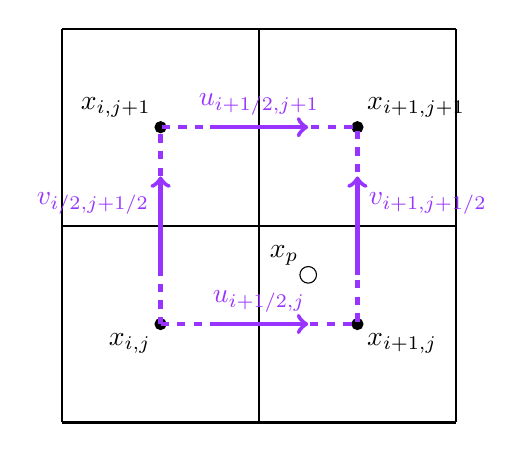
\begin{tikzpicture}[declare function={a=2.5;}]
        \coordinate (A) at (0,0);
        \coordinate (B) at (a,0);
        \coordinate (C) at (2*a,0);
        \coordinate (D) at (0,a);
        \coordinate (E) at (a,a);
        \coordinate (F) at (2*a,a);
        \coordinate (G) at (0,2*a);
        \coordinate (H) at (a,2*a);
        \coordinate (I) at (2*a,2*a);
        \draw[thick] (A) -- (C);
        \draw[thick] (D) -- (F);
        \draw[thick] (G) -- (I);        
        \draw[thick] (A) -- (G);
        \draw[thick] (B) -- (H);
        \draw[thick] (C) -- (I);     
        \filldraw[black] (a/2,a/2) circle (2pt) node[anchor = north east]{$x_{i,j}$};
        \filldraw[black] (3*a/2,a/2) circle (2pt) node[anchor = north west]{$x_{i+1,j}$};
        \filldraw[black] (a/2,3*a/2) circle (2pt) node[anchor = south east]{$x_{i,j+1}$};
        \filldraw[black] (3*a/2,3*a/2) circle (2pt) node[anchor = south west]{$x_{i+1,j+1}$};
        \draw (10*a/8,6*a/8) circle (3pt) node[anchor = south east]{$x_p$};
        % \draw[->,ultra thick,purple] (-a/4,a/2) -- node[above] {$u_{i-1/2,j}$}(a/4, a/2);
        \draw[->,ultra thick,purple] (3*a/4,a/2) --node[above] {$u_{i+1/2,j}$} (5*a/4, a/2);
        % \draw[->,ultra thick,purple] (7*a/4,a/2) -- node[above] {$u_{i+3/2,j}$}(9*a/4, a/2);
        % \draw[->,ultra thick,purple] (a/4,a) -- node[above] {$u_{i,j+1/2}$}(3*a/4, a);
        % \draw[->,ultra thick,purple] (5*a/4,a) -- node[above] {$u_{i,j+3/2}$}(7*a/4, a);
        % \draw[->,ultra thick,purple] (-a/4,3*a/2) -- node[above] {$u_{i-1/2,j+1}$}(a/4, 3*a/2);
        \draw[->,ultra thick,purple] (3*a/4,3*a/2) -- node[above] {$u_{i+1/2,j+1}$}(5*a/4, 3*a/2);
        % \draw[->,ultra thick,purple] (7*a/4,3*a/2) --node[above] {$u_{i+1/2,j+1}$} (9*a/4, 3*a/2);
        % \draw[->,ultra thick,purple] (a/4,0) -- node[above] {$u_{i,j+1/2}$}(3*a/4, 0);
        % \draw[->,ultra thick,purple] (5*a/4,0) -- node[above] {$u_{i+1,j-1/2}$}(7*a/4, 0);
        % \draw[->,ultra thick,purple] (a/4,2*a) -- node[above] {$u_{i+1,j+1/2}$}(3*a/4, 2*a);
        % %\draw[arrow] (pro1) -- node[right] {After convergence} (pro2);
        % \draw[->,ultra thick,purple] (5*a/4,2*a) --node[above] {$u_{i+1,j+3/2}$} (7*a/4, 2*a);
        \draw[->, ultra thick, purple] ( a/2,3*a/4) -- node[above left] {$v_{i/2,j+1/2}$} (a/2,5*a/4);
        \draw[->, ultra thick, purple] ( 3*a/2,3*a/4) -- node[above right] {$v_{i+1,j+1/2}$} (3*a/2,5*a/4);
        %\node at (a/2,a/2) {$x_{i,j}$};
        \draw[ultra thick, dashed, purple] (a/2,a/2) -- (3*a/2,a/2) -- (3*a/2,3*a/2) -- (a/2,3*a/2) -- cycle;
    \end{tikzpicture}
    \label{fig:intTwoNeigh}
    \caption{Velocity values used in the closest-neighbor interpolation method for interpolating from the Eulerian grid to $\xp$.}
    \end{subfigure}

    
    \begin{subfigure}[b]{0.4\textwidth}
    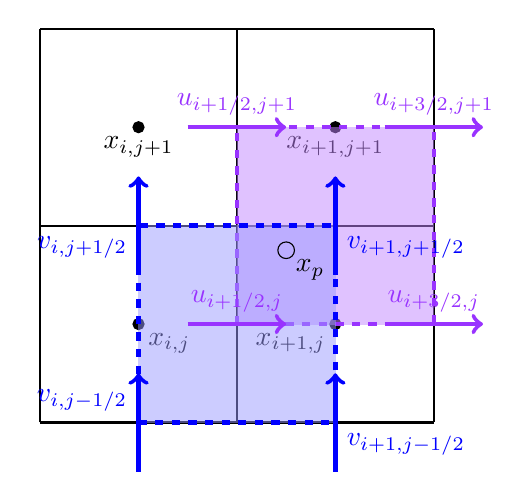
\begin{tikzpicture}[declare function={a=2.5;}]
        \coordinate (A) at (0,0);
        \coordinate (B) at (a,0);
        \coordinate (C) at (2*a,0);
        \coordinate (D) at (0,a);
        \coordinate (E) at (a,a);
        \coordinate (F) at (2*a,a);
        \coordinate (G) at (0,2*a);
        \coordinate (H) at (a,2*a);
        \coordinate (I) at (2*a,2*a);
        \draw[thick] (A) -- (C);
        \draw[thick] (D) -- (F);
        \draw[thick] (G) -- (I);        
        \draw[thick] (A) -- (G);
        \draw[thick] (B) -- (H);
        \draw[thick] (C) -- (I);     
        \filldraw[black] (a/2,a/2) circle (2pt) node[anchor = north west]{$x_{i,j}$};
        \filldraw[black] (3*a/2,a/2) circle (2pt) node[anchor = north east]{$x_{i+1,j}$};
        \filldraw[black] (a/2,3*a/2) circle (2pt) node[anchor = north]{$x_{i,j+1}$};
        \filldraw[black] (3*a/2,3*a/2) circle (2pt) node[anchor = north]{$x_{i+1,j+1}$};
        % \draw[->,ultra thick,purple] (-a/4,a/2) -- node[above] {$u_{i-1/2,j}$}(a/4, a/2);
        
        %\draw[->,ultra thick,purple] (a/4,0) -- node[above] {$u_{i,j+1/2}$}(3*a/4, 0);
        %\draw[->,ultra thick,purple] (5*a/4,0) -- node[above] {$u_{i+1,j-1/2}$}(7*a/4, 0);
        %\draw[->,ultra thick,purple] (a/4,2*a) -- node[above] {$u_{i+1,j+1/2}$}(3*a/4, 2*a);
        %\draw[arrow] (pro1) -- node[right] {After convergence} (pro2);
        %\draw[->,ultra thick,purple] (5*a/4,2*a) --node[above] {$u_{i+1,j+3/2}$} (7*a/4, 2*a);
        \shade[shading=axis, top color=purple!60, bottom color=purple!60, opacity =0.5] (a,a/2) -- (a,3*a/2) -- (2*a,3*a/2) -- (2*a,a/2) -- cycle;
        \draw[ultra thick,dashed, purple](a,a/2) -- (a,3*a/2) -- (2*a,3*a/2) -- (2*a,a/2) -- cycle;
        \shade[shading=axis, top color=blue!40, bottom color=blue!40, opacity =0.5] (a/2,0) -- (3*a/2,0) -- (3*a/2,a) -- (a/2,a) -- cycle;
        \draw[ultra thick,dashed, blue](a/2,0) -- (3*a/2,0) -- (3*a/2,a) -- (a/2,a) -- cycle;
        \draw[->,ultra thick,purple] (3*a/4,a/2) --node[above] {$u_{i+1/2,j}$} (5*a/4, a/2);
        \draw[->,ultra thick,purple] (7*a/4,a/2) -- node[above] {$u_{i+3/2,j}$}(9*a/4, a/2);
        %\draw[->,ultra thick,purple] (a/4,a) -- node[above] {$u_{i,j+1/2}$}(3*a/4, a);
        %\draw[->,ultra thick,purple] (5*a/4,a) -- node[above] {$u_{i,j+3/2}$}(7*a/4, a);
        %\draw[->,ultra thick,purple] (-a/4,3*a/2) -- node[above] {$u_{i-1/2,j+1}$}(a/4, 3*a/2);
        \draw[->,ultra thick,purple] (3*a/4,3*a/2) -- node[above] {$u_{i+1/2,j+1}$}(5*a/4, 3*a/2);
        \draw[->,ultra thick,purple] (7*a/4,3*a/2) --node[above] {$u_{i+3/2,j+1}$} (9*a/4, 3*a/2);
        \draw[->,ultra thick, blue] (a/2,3*a/4) -- node[below left] {$v_{i,j+1/2}$}(a/2,5*a/4);
        \draw[->,ultra thick, blue] (3*a/2,-a/4) -- node[below right] {$v_{i+1,j-1/2}$}(3*a/2,a/4);
        \draw[->,ultra thick, blue] (a/2,-a/4) -- node[above left]{$v_{i,j-1/2}$} (a/2,a/4);
        \draw[->,ultra thick, blue] (3*a/2,3*a/4) -- node[below right] {$v_{i+1, j+1/2}$} (3*a/2,5*a/4);
        \draw (10*a/8,7*a/8) circle (3pt) node[anchor = north west]{$x_p$};
        %\node at (a/2,a/2) {$x_{i,j}$};
    \end{tikzpicture}
    \label{fig:bilinearInt}
     \caption{Velocity values used in the bilinear interpolation.}
    \end{subfigure}
    \caption{Interpolation with face values.}
\end{figure}
Once again we use the top hat functions we defined earlier.
For the two-neighbor interpolation we use the velocity $u$ in $\x$ direction and the velocity $v$ in $y$ direction. As the name suggests we use the two neighboring velocities, see figure \subref{fig:intTwoNeigh}. We use two top hat functions for the $\x$-face velocity
\begin{align}
    \ip_{i+1/2,j}^{T} &= \ifg_{i+1/2} \ifg_j \\
    \u_{g,p} &= \ip_{i+1/2,j}^{T} (\xp) \u_{g_{i+1/2,j}} +  \ip_{i+1/2,j+1}^{TS} (\xp) \u_{g_{i+1/2,j+1}} \\
    v_{g,p} &= \ip_{i,j+1/2}^{T} (\xp) \u_{g_{i,j+1/2}} +  \ip_{i+1,j+1/2}^{TS} (\xp) \u_{g_{i+1,j+1/2}}.
\end{align}

The second option is to use face bilinear interpolation as shown in figure \subref{fig:bilinearInt}. Compared to the closest neighbor interpolation we now double the cell faces used to four per direction. 
For both the $x$ and the $y$ direction we use the encompassing faces for the interpolation operators
\begin{equation*}
    \ip_{i+1/2,j}^S = \ip^x_{i+1/2} \ip^y_{j} \qquad \ip_{i,j+1/2}^S = \ip^x_i \ip^y_{j+1/2}
\end{equation*}
and then have the interpolated velocity
\begin{align*}
    \u_{g,p} = \ip^S_{i+1/2,j} (\xp) \u_{g_{i+1/2,j}} + \ip_{i+3/2,j}^S (\xp) \u_{g_{i+3/2,j}} + \ip_{i+3/2,j+1}^S (\xp) \u_{g_{i+3/2,j+1}} + \ip^S_{i+1/2,j+1}(\xp)\u_{g_{i+1/2,j+1}}\\
    v_{g,p} =  \ip^S_{i,j+1/2} (\xp) v_{g_{i,j+1/2}} + \ip^S_{i+1,j+1/2} (\xp) v_{g_{i+1,j+1/2}} + \ip^S_{i+1,j-1/2} (\xp) v_{g_{i+1,j-1/2}}+\ip^S_{i,j-1/2} (\xp) v_{g_{i,j-1/2}}.
\end{align*}
%\color{gray}
\Todo{Which one is used?}

For the momentum continuity equation, we also need the gradient of the interpolation operator.
The gird property $\gp$ mapped to the particle location $\xp$ is
\begin{equation*}
    \nabla \gp_p = \sum_{\xi =1}^{N} \nabla \ip_{\xi}(\xp) \gp_{\xi} + \sum_{\xi = 1}^N \ip_{\xi} ( \xp) (\nabla \gp)_\xi = \sum_{\xi =1}^N \ip_{\xi} ( \xp) (\nabla \gp)_\xi.
\end{equation*}
Here the particle position is fixed leading to the second equality.
Furthermore can also map the gradient of a grid property $\gp$ to and from the particle
\begin{equation*}
    \nabla \ip_\zeta (\xp) \cdot \sum_{\xi =1}^8 \ip_\xi ( \xp ) \nabla \gp_\xi = \sum_{i=1}^8 \nabla \ip_\zeta ( \xp ) \cdot [\ip_\xi (\xp) \nabla \gp_\xi].
\end{equation*}
To simplify the equation we first look a the product of an interpolation operator with the gradient of an interpolation operator
\begin{equation*}
    \sum_\xi \ip_\xi \nabla \ip_\zeta = \sum_\xi \ip_{x_\zeta} \ip_{y_\zeta} \ip_{z_\zeta} \begin{pmatrix}
        \frac{\partial \ip_{x_\xi}}{\partial x} \ip_{y_\xi} \ip_{z_\xi} \\
        \frac{\partial \ip_{y_\xi}}{\partial y} \ip_{x_\xi} \ip_{z_\xi} \\
        \frac{\partial \ip_{z_\xi}}{\partial z} \ip_{x_\xi} \ip_{y_\xi}
    \end{pmatrix}.
\end{equation*}
We can apply the orthogonality property from equation \eqref{eq:ipOrtho} and then receive
\begin{equation*}
    \nabla \ip_\zeta ( \xp ) \cdot \sum_{\xi=1}^8 \ip_\xi ( \xp ) \nabla \gp_\xi = \ip_\zeta \left[ \dfrac{\partial \ip_{x_\zeta}}{\partial x} \boldsymbol{e}_x + \dfrac{\partial \ip_{y_\zeta}}{\partial y} \boldsymbol{e}_y + \dfrac{\partial \ip_{z_\zeta}}{\partial z} \boldsymbol{e}_z\right].
\end{equation*}


\color{black}

\subsection{Numerical Solution without damping terms}
The interpolation operators introduced in the previous section are used in the \MP method to map particle properties between the Eulerian grid and the particle positions.
The method can be roughly split into the the following three steps in each time step.
First the method calculates the provisional particle positions based on the previous velocity and particle positions.
These positions are used to map the properties like particle volume fraction to the Eulerian grid.
Then the momentum and continuity equation are solved on the Eulerian map.
Derivative terms for example for the solid stress are mapped back to the particles and used to calculate the advanced particle positions.
This completes the completes the time step.
In the following we will derive each step and look at the implicit approximations used.

For the numerical solution we use the parcels mentioned above. As per the assumption made in equation \eqref{eq:partConservation}, the number of particles in a volume is conserved in particle phase space. 
Therefor the parcels have a constant number of particles.
For now we assume that a particle's mass is constant.
Particle positions are then calculated by
\begin{equation}
    \label{eq:MPposition}
    \xp^{n+1} = \xp^{n} + \Delta t \up^{n+1}, \ n \in \mathbb{N} \qquad \xp^{0} = \x_0
\end{equation}
and the velocity is updated by integrating the acceleration \eqref{eq:accel}
% \Todo{Anpassen auf altes Paper}
\begin{align}
    \label{eq:errVel}
    \dfrac{\up^{n+1} - \up^{n}}{\Delta \tvar} &= \d (\upi^{n+1} -
    \up^{n+1})  - \dfrac{1}{\rp} \nabla_{\xp} \p_p^{n+1} - \dfrac{1}{\rp \pvf} \nabla_{\xp} \scs^{n+1} - \g \\
    \Leftrightarrow \up^{n+1} &= \dfrac{\up^n + \Delta \tvar \left[ \d_p \up^{n+1} - \dfrac{1}{\rp} \nabla_{\xp} \p_p^{n+1} - \dfrac{1}{\rp \pvf} \nabla_{\xp} \scs^{n+1} - \g \right]}{1 + \Delta \tvar \d} .
\end{align}

In the following we will restrict ourselves to the one dimensional case for easier reading. 
For the gradients we use a differential quotient 
\begin{equation}
\label{eq:MPvelocity}
    \up^{n+1} = \dfrac{\up^n + \Delta \tvar \left[\d_p \tilde{u_{G,p}} - \g - \dfrac{1}{\rp} \left(\dfrac{\tilde{\p}_{i+1} - \tilde{\p}_i}{\Delta \x} \right)_p - \dfrac{1}{\rp \pvf} \left( \dfrac{\tilde{\ss}_{i+1} - \tilde{\ss}_i}{\Delta \x}\right)_p \right]}{1 + \Delta \tvar \d_p}
\end{equation}
Variables marked with a tilde $\tilde{\cdot}$ are implicit approximations to the advanced-time step. They as well as the interphase momentum transfer will be defined in the following.

The equations for updating the position \eqref{eq:MPposition} and velocity \eqref{eq:MPvelocity} are used at the end of a time step to calculate the new particle velocities and positions.
These two equations are the first of eight equations.
In total we will need eight equations which we will derive in the following.
We start by applying the finite differences scheme to the fluid continuity equation
\begin{equation}
    \label{eq:gasContDisc}
    \dfrac{(\fvf \rf)_i^{n+1} - (\fvf \rf)_i^n}{\Delta \tvar} + \dfrac{(\fvf \rf \uf)_{i+\frac{1}{2}}^{n+1}- \fvf \rf \uf)_{i-\frac{1}{2}}^{n+1}}{\Delta \xp} = 0,
\end{equation}
and the momentum equation
\begin{equation}
    \label{eq:discMom}
    \dfrac{(\fvf \rf \uf)_{i+\frac{1}{2}}^{n+1}- (\fvf \rf \uf)_{i+\frac{1}{2}}^{n}}{\Delta \tvar} + \dfrac{(\fvf \rf \uf^2)^n_{i+1}-\fvf \rf \uf^2)^n_{i}}{\Delta \xp} + \dfrac{\tilde{\p}_{i+1}-\tilde{p}_i}{\Delta \xp} = - \F_{i+\frac{1}{2}}-\dfrac{((\fvf \rf)_i^n + (\fvf \rf)_{i+1}^n)\g}{2}.
\end{equation}
% \Todo{Does this actually make sense?}


To approximate the convective flux $\fvf \rf \uf^2$ we it into the mass flux and the fluid velocity.
Since the mass flux is only known at the cell faces we use a central approximation scheme for the cell center. 
For the velocity, we use an upwind approximation scheme

\begin{align*}
    (\fvf \rf \uf^2)_i^n = \dfrac{\m_{i+\frac{1}{2}}+\m_{i-\frac{1}{2}}}{2} \cdot
    \begin{cases}
        (\uf)^n_{i- \frac{1}{2}} & \text{if } \m_{i-\frac{1}{2}} + \m_{i+\frac{1}{2}} > 0 \\
        (\uf)^n_{i+ \frac{1}{2}} & \text{if } \m_{i-\frac{1}{2}} + \m_{i+\frac{1}{2}} < 0
    \end{cases}
\end{align*}

with the mass flux calculated at the matching face and the fluid velocity calculated with the neighboring volume fraction times the fluid density
\begin{align*}
    m_{i+\frac{1}{2}} = (\fvf \rf \uf)^n_{i+\frac{1}{2}} \qquad (\uf)_{i+\frac{1}{2}}^n = \dfrac{2 (\fvf \rf \uf)_{i+\frac{1}{2}}}{(\fvf \rf)_{i} + (\fvf \rf)_{i+1}^n}.
\end{align*}


For the pressure we use the ideal gas assumption from above \eqref{eq:gasDensReal} that fluid pressure and the density are related we have
\begin{equation}
    \p = c_1 \rf^\gamma = c_1 \left( \dfrac{R}{\fvf}\right)^\gamma = c_1 \left( \dfrac{R}{1 - \pvf}\right)^\gamma \quad \text{with} \quad R \coloneq \fvf \rf.
\end{equation}
Because the pressure is nonlinear we use an implicit approximation to the gas pressure. 
A first order Taylor expansion around $((\fvf \rf)^{n},\pvf^n)$  evaluated at time-step $n+1$ yields
\begin{equation}
\label{eq:pTaylor}
    \p^{n+1} = \p^n + \dfrac{\partial \p}{\partial (\fvf \rf)}\bigg|^n \left[ (\fvf \rf )^{n+1} - (\fvf \rf)^n \right] +\dfrac{\partial \p}{\partial \pvf}\bigg|^n \left[ \pvf  ^{n+1} - \pvf^n \right].
\end{equation}
Both derivatives can be explicitly calculated by
\begin{equation*}
    \dfrac{\partial \p}{\partial (\fvf \rf)} = \dfrac{\partial \p}{\partial R} = c_1 \gamma \left( \dfrac{R}{\fvf}\right)^{\gamma -1} \dfrac{1}{\fvf}= \dfrac{\gamma}{R} \p
\end{equation*}
and
\begin{equation*}
    \dfrac{\partial \p}{\partial \pvf} = c_1 \gamma \dfrac{1}{1- \pvf} \left( \dfrac{R}{1 - \pvf}\right)^\gamma = \dfrac{\gamma}{1-\pvf} \p.
\end{equation*}
Inserting both back into the Taylor expansion \eqref{eq:pTaylor}
\begin{equation}
    \p_i^{n+1} = \p^n \left( 1 + \gamma \left[\dfrac{(\fvf \rf)^{n+1} - (\fvf \rf)^{n}}{(\fvf \rf)^n} + \dfrac{\widetilde{\pvf} - \pvf^n}{1 - \pvf^n} \right] \right)
\end{equation}
with $\p_i^{n}$ approximated by
\begin{equation*}
    c_1 \coloneq \dfrac{\p_{ref}}{\rgref^\gamma} \quad  \Rightarrow \quad \p_i^n = \p_{ref} \left[ \dfrac{(\fvf \rf )_i^n}{(1- \pvfi^n)\rgref} \right]^\gamma.
\end{equation*}
with $\p_{ref}$ and $\rgref$ at some reference state. For $\pvfi^n$ we use the discretization
\begin{equation*}
    \pvfi^n = \dfrac{1}{\Delta x} \sum_p \ip_i(\x_p^n) \dfrac{\m_p}{\rp} \Np.
\end{equation*}
$\pvf^{n+1}$ is approximated by $\widetilde{\pvf}$ and will be discussed later. 
\Todo{Wandeffekte?}

For mapping properties defined at the faces back to the parcels, we define the provisional parcel position
\begin{equation}
    \label{eq:provPartPos}
    \xpp = \xp^n + \up^n \Delta \tvar.
\end{equation}
and use the cell-face interpolation function e.g.
\begin{equation}
    \label{eq:cellFaceInterpolation}
    \left( \dfrac{\tilde{\p_{i+1}} - \tilde{\p_{i}}}{\Delta x} \right)_p = \sum_i \ifg_{i+ \frac{1}{2}} (\xpp ) \frac{\tilde{p}_{i+1} - \tilde{p}_i}{\Delta x}.
\end{equation}
For the approximation of the advanced-time solids stress we again use a an linearly implicit approximation, the Taylor expansion applied to \eqref{eq:solidStress} around $\pvfi^n$ evaluated at $\tilde{\pvfi}$
\begin{align}
    \ss_i^{n+1} &= \ss_i^n + \dfrac{\partial \ss}{\partial \pvf}\bigg|_n  (\pvfi^{n+1} - \pvfi^n)  \qquad \dfrac{\partial \ss}{\partial \pvf}\bigg|_n = P_s \dfrac{\pvfcp}{\pvf^2} \left( \dfrac{\pvfcp}{\pvf} -1 \right)^{-2}\\
    \Rightarrow \tilde{\ss}_i &= \ss_i^n + P_s\dfrac{\pvfcp}{(\pvfcp - \pvf)^2} (\tilde{\pvf}- \pvfi^n).
\end{align}
To approximate the volume fraction for each parcel we first need to get it at the cell faces before we can interpolate it to the parcels. 
For cell faces we use properties from the Eulerian grid
\begin{equation}
    \label{eq:interpolationPVFCellFace}
    \pvf_{i+ \frac{1}{2}} = \dfrac{1}{\Delta x} \sum_p \ifg_{i+\frac{1}{2}} (\xpp ) \Np \dfrac{\m_p}{\rp}
\end{equation}
and then weight the volume fraction by the interpolation function to get the volume fraction at the provisional parcel position
\begin{equation}
    \label{eq:interpolatePPP}
    \pvfp = \sum_i \ifg_{i+\frac{1}{2}} (\xpp) \pvf_{i+\frac{1}{2}}.
\end{equation}

To verify the discretizations above, we look at whether the parcel momentum is conserved. 
We multiply the discretized momentum equation \eqref{eq:discMom} by $\Np \mp$  and sum over all parcels
\begin{align*}
    \sum_p \Np \mp \dfrac{\up^{n+1}-\up^n}{\Delta \tvar} =& - \sum_p \Np \mp \g - \sum_p \dfrac{\Np \mp}{\rp} \left( \dfrac{\tilde{\p}_{i+1}- \tilde{\p}_i}{\Delta \x}\right)_p + \sum_p D_p \Np \mp (\tilde{\ugp} - \up^{n+1}) \\
    &- \sum_p \dfrac{\Np \mp}{\rp \pvfp} \left( \dfrac{\tilde{\ss}_{i+1}-\tilde{\ss}_i}{\Delta \x}\right)_p.
\end{align*}
Using the previous definitions the last term becomes
\begin{align*}
    \sum_p \dfrac{\Np \mp}{\rp \pvf} \left( \dfrac{\tilde{\ss}_{i+1}-\tilde{\ss}_i}{\Delta \x}\right)_p \stackrel{\eqref{eq:cellFaceInterpolation}}{=} \sum_p \dfrac{\Np \mp}{\rp \pvf} \sum_i \ifg_{i+\frac{1}{2}}(\xpp) \dfrac{\tilde{\ss}_{i+1}-\tilde{\ss_i}}{\Delta \x} = \sum_i \sum_p \left( \dfrac{\Np \mp}{\rp} \ifg_{i+\frac{1}{2}} ( \xpp)\right)\dfrac{\tilde{\ss}_{i+1}- \tilde{\ss}_i}{\pvf_{i+\frac{1}{2}} \Delta \x}.
\end{align*}
For the last step we used
\begin{equation*}
    \pvf \stackrel{\eqref{eq:interpolatePPP}}{=} \sum_{i}  \ifg_{i+\frac{1}{2}} (\xpp) \pvf_{i+\frac{1}{2}} = \pvf_{i+\frac{1}{2}} \qquad \iff \qquad \ifg_{i+\frac{1}{2}} (\xpp) = 1
\end{equation*}
Using \eqref{eq:interpolationPVFCellFace} gives us
\begin{align*}
    \sum_i \sum_p \left( \dfrac{\Np \mp}{\rp} \ifg_{i+\frac{1}{2}} ( \xpp)\right)\dfrac{\tilde{\ss}_{i+1}- \tilde{\ss}_i}{\frac{1}{\Delta \x}\sum_p \dfrac{\Np \mp}{\rp} \ifg_{i+\frac{1}{2}} ( \xpp) \Delta \x} %= \sum_i \tilde{\ss}_{i+1}-\tilde{\ss}_i 
    = \sum_{i=0}^{N} \tilde{\ss}_{i+1} - \tilde{\ss}_i = \tilde{\ss}_N - \tilde{\ss}_0,
\end{align*}
which are the boundary sources thus proving momentum conservation.
Here we only look at the one dimensional case but this can be extended to two and three-dimensional cases with their respective boundary terms. Thus the implicit approximation conserves the momentum.

Similarly, for the advanced-time gas velocity, we use the interpolation to the faces
\begin{equation*}
    \tilde{\ufp} = \sum_i \ifg_{i+\frac{1}{2}} (\xpp) \dfrac{2 (\fvf \rf \uf)_{i+\frac{1}{2}}^{n+1}}{(\fvf \rf)_i^n + (\fvf \rf)_{i+1}^n}.
\end{equation*}
This definition is also used in the particle drag function. 
For the density and the fluid phase fraction at the provisional parcel position, we avoid calculation of extra parameters by using known quantities and interpolate to the cell middle
\begin{align*}
    \rf = \dfrac{\fvf \rf}{\fvf} = \dfrac{\fvf \rf}{1-\pvf} \quad
    \Rightarrow \quad \rfp = \sum_i \ip_i (\xpp) \dfrac{(\fvf \rf)_i^n}{1 - \pvfi^n}
\end{align*}
for the fluid volume fraction we use an upwind scheme
\begin{align*}
    \fvf = \begin{cases}
        \sum_i \ifg_{i+\frac{1}{2}} (\xpp) (1 - \pvf_{i+1}^n) & \text{if } \up^n > 0 \\
        \sum_i \ifg_{i+\frac{1}{2}} (\xpp) (1 - \pvfi^n) & \text{if } \up^n \leq 0
    \end{cases}
\end{align*}

To achieve momentum conservation we group the remaining terms into the momentum exchange term
\begin{equation*}
    \F_{i+\frac{1}{2}} = \left( \sum_p \ifg_{i+\frac{1}{2}} (\xpp) \left. \left[ D_p (\tilde{\ugp} - \up^{n+1} ) - \dfrac{1}{\rp} \left( \dfrac{\tilde{\p}_{i+1} - \tilde{p}_i}{\Delta x}\right)_p \right] \Np \mp \right) \middle / \right. \Delta \x.
\end{equation*}
This ensures the momentum in conserved.

The key feature of the \MP method lies in the calculation of the particle volume fraction $\pvf$ for each cell. 
The advanced particle volume fraction $\tilde{\pvfi}$ closely approximates $\pvf$.

So far we have given approximations to the grid values, e.g. $\ss$ and $\p$.
Once the grid values are calculated we can approximate the new particle positions by using the velocity calculated in equation \eqref{eq:MPvelocity} and approximate the new particle positions. 
We then map the particle properties to their positions.
\color{ForestGreen}
First we derive the discretized fluid-phase momentum equation. 
We recall the particle velocity
\begin{equation}
    \label{eq:advVelocity}
    \up^{n+1} = \dfrac{\up^n + \Delta \tvar \left[\d_p \tilde{u_{G,p}} - \g - \dfrac{1}{\rp} \left(\dfrac{\tilde{\p}_{i+1} - \tilde{\p}_i}{\Delta \x} \right)_p - \dfrac{1}{\rp \pvf} \left( \dfrac{\tilde{\ss}_{i+1} - \tilde{\ss}_i}{\Delta \x}\right)_p \right]}{1 + \Delta \tvar \d_p}
\end{equation}
and use it to replace $\up^{n+1}$ in the momentum exchange term $\F_{i+\frac{1}{2}}$ and summarize the pressure and implicit velocity terms
\begin{align*}
    \hspace{-0.5cm} \F_{i+\frac{1}{2}} &= \left( \sum_p \ifg_{i+\frac{1}{2}} (\xpp) \left. \left[ D_p (\tilde{\ugp} - 
    \up^{n+1} 
    ) - \dfrac{1}{\rp} \left( \dfrac{\tilde{\p}_{i+1} - \tilde{p}_i}{\Delta x}\right)_p \right] \Np \mp \right) \middle / \right. \Delta \x \\
    &=  \dfrac{1}{\Delta \x} \left( \sum_p \ifg_{i+\frac{1}{2}} (\xpp) \left[ D_p \left(\tilde{\ugp} - 
    \dfrac{1}{1 + \Delta \tvar \d_p}    
    \left( \up^n + \Delta \tvar \left[\d_p \tilde{u_{G,p}} - \g - \dfrac{1}{\rp} \left(\dfrac{\tilde{\p}_{i+1} - \tilde{\p}_i}{\Delta \x} \right)_p - \dfrac{1}{\rp \pvf} \left( \dfrac{\tilde{\ss}_{i+1} - \tilde{\ss}_i}{\Delta \x}\right)_p \right] \right) \right) \right. \right. \\
    & \left. \left. - \dfrac{1}{\rp} \left( \dfrac{\tilde{\p}_{i+1} - \tilde{p}_i}{\Delta x}\right)_p \Np \mp \right) \right] \\
    &=  \dfrac{1}{\Delta \x} \left( \sum_p \ifg_{i+\frac{1}{2}} (\xpp) \left[ D_p \left(-  \dfrac{1}{1 + \Delta \tvar \d_p} \left(   \up^n - \tilde{\u}_{G,p}     + \dfrac{1}{\rp} \left(\dfrac{\tilde{\p}_{i+1} - \tilde{\p}_i}{\Delta \x} \right)_p + \Delta \tvar \left[ - \g - \dfrac{1}{\rp \pvf} \left( \dfrac{\tilde{\ss}_{i+1} - \tilde{\ss}_i}{\Delta \x}\right)_p \right] \right) \right) \Np \mp \right]\right)
\end{align*}
We then use the former equation to substitute $\F_{i+\frac{1}{2}}$ from the discrete momentum equation \eqref{eq:discMom} thus having
\begin{align*}
    &\dfrac{(\fvf \rf \uf)_{i+\frac{1}{2}}^{n+1}- (\fvf \rf \uf)_{i+\frac{1}{2}}^{n}}{\Delta \tvar} + \dfrac{(\fvf \rf \up^2)^n_{i+1}-(\fvf \rf \up^2)^n_{i}}{\Delta \xp} + \dfrac{\tilde{\p}_{i+1}-\tilde{p}_i}{\Delta \xp} \\
    &= \dfrac{1}{\Delta \x} \left( \sum_p \ifg_{i+\frac{1}{2}} (\xpp) \left[ D_p \left(- 
    \dfrac{1}{1 + \Delta \tvar \d_p} \left(
    \up^n - \tilde{\u}_{G,p} 
    + \dfrac{1}{\rp} \left(\dfrac{\tilde{\p}_{i+1} - \tilde{\p}_i}{\Delta \x} \right)_p + \Delta \tvar \left[ - \g - \dfrac{1}{\rp \pvf} \left( \dfrac{\tilde{\ss}_{i+1} - \tilde{\ss}_i}{\Delta \x}\right)_p \right] \right) \right) \Np \mp \right] \right)\\
    &-\dfrac{((\fvf \rf)_i^n + (\fvf \rf)_{i+1}^n)\g}{2}.
\end{align*}
Looking just at the pressure terms by rearranging the terms and using the interpolation property $\ifg_{i+\frac{1}{2}} (\xpp) \sum_j \ifg_{j+\frac{1}{2}} (\xpp) = \ifg_{i+\frac{1}{2}} (\xpp)$ to
\begin{align*}
    \dfrac{\tilde{\p}_{i+1}-\tilde{\p}_i}{\Delta \xp} = \sum_p \ifg_{i+\frac{1}{2}} (\xpp) \dfrac{\Np \mp}{\rp \Delta \x (1 + \Delta \tvar \d_p)} \left( \dfrac{\tilde{\p}_{i+1} - \tilde{\p}_i}{\Delta \x} \right)_p \\
\Leftrightarrow \left( \dfrac{\tilde{\p}_{i+1} - \tilde{\p}_i}{\Delta \x} \right)
 \left( 1 - \sum_p \ifg_{i+\frac{1}{2}} (\xpp) \dfrac{\Np \mp}{\rp \Delta \x (1 + \Delta \tvar \d_p)} \right) = 0.
\end{align*}


For the solid stress we again use the interpolation property and receive
\begin{align*}
    0 &= - \sum_p \ifg_{i+\frac{1}{2}} (\xpp) \d_p \dfrac{1}{1+ \Delta \tvar \d_p} \Delta \tvar \dfrac{1}{\rp \pvf} \left( \dfrac{\tilde{\ss}_{i+1} - \tilde{\ss}_{i}}{\Delta \x} \right)_p \\
    \Leftrightarrow
    0 &= - \dfrac{1}{\Delta x \theta_{i+\frac{1}{2}}} \sum_{p} \ifg_{i+\frac{1}{2}} (\xpp) \sum_p \left[ \Np \dfrac{\mp}{\rp} \ifg_{i+\frac{1}{2}} (\xpp) \dfrac{\Delta \tvar \d_p}{1 + \Delta \tvar \d_p}  \right] \dfrac{\tilde{\ss}_{i+1} - \tilde{\ss}_{i}}{\Delta \x}.
\end{align*}
Lastly we look at the terms for the advanced-time gas velocity and using the the interpolation property and the approximation $(\pvf \rf)_i^n + (\pvf \rf)_{i+1}^n = 2 (\pvf \rf)_{i+\frac{1}{2}}^n$
\begin{align*}
    0 &= - \dfrac{1}{\Delta \x} \sum_p \ifg_{i+\frac{1}{2}} ( \xpp ) \d_p \tilde{\ufp} \dfrac{1}{1+\Delta \tvar \d_p} \Np \mp  \\
    \Leftrightarrow 0 &= - \dfrac{1}{\Delta \x} \sum_p \d_p 
    \sum_i \ifg_{i+\frac{1}{2}} (\xpp) \dfrac{2 (\pvf \rf \uf)_{i+\frac{1}{2}}^{n+1}}{(\pvf \rf)_i^n + (\pvf \rf)_{i+1}^n} \dfrac{1}{1+\Delta \tvar \d_p} \Np \mp \\
    \Leftrightarrow 0 &= 
    \dfrac{1}{\Delta \x (\pvf \rf)_{i+\frac{1}{2}}^n} \sum_p \left[ \Np \mp \ifg_{i+\frac{1}{2}} (\xpp) \frac{\d_p}{1+ \Delta \tvar \d_p}\right] (\pvf \rf)_{i+\frac{1}{2}}^n.
\end{align*}

\color{black}
Combining these terms we have fluid momentum equation
\begin{equation}
\begin{aligned}
\label{eq:momentumEquationFluidDisc}
    &\dfrac{(\fvf \rf \uf)_{i+\frac{1}{2}}^{n+1}- (\fvf \rf \uf)_{i+\frac{1}{2}}^{n}}{\Delta \tvar} + \dfrac{(\fvf \rf \up^2)^n_{i+1}-\fvf \rf \up^2)^n_{i}}{\Delta \xp}
    +  \left( \dfrac{\tilde{\p}_{i+1} - \tilde{\p}_i}{\Delta \x} \right) 
    \left( 1 - \sum_p \ifg_{i+\frac{1}{2}} (\xpp) \dfrac{\Np \mp}{\rp \Delta \x (1 + \Delta \tvar \d_p)} \right) \\
    &=
    \dfrac{1}{\Delta \x (\pvf \rf)_{i+\frac{1}{2}}^n} \sum_p \left[ \Np \mp \ifg_{i+\frac{1}{2}} (\xpp) \frac{\d_p}{1+ \Delta \tvar \d_p}\right] (\pvf \rf)_{i+\frac{1}{2}}^n
    + \dfrac{1}{\Delta \x} \sum_p \left[ \Np \dfrac{\mp}{\rp} \ifg_{i+\frac{1}{2}} (\xpp) \dfrac{\d_p (\up^n - \Delta \tvar \g)}{1 + \Delta \tvar \d_p^n}\right] \\
    &- \dfrac{1}{\Delta x \theta_{i+\frac{1}{2}}} \sum_{p} \ifg_{i+\frac{1}{2}} (\xpp) \sum_p \left[ \Np \dfrac{\mp}{\rp} \ifg_{i+\frac{1}{2}} (\xpp) \dfrac{\Delta \tvar \d_p}{1 + \Delta \tvar \d_p}  \right] \dfrac{\tilde{\ss}_{i+1} - \tilde{\ss}_{i}}{\Delta \x}    
    -\dfrac{((\fvf \rf)_i^n + (\fvf \rf)_{i+1}^n)\g}{2}.
\end{aligned}
\end{equation}
We summarize terms that only depend on known information and have
\begin{align*}
    \dfrac{(\fvf \rf \uf)_{i+\frac{1}{2}}^{n+1}- (\fvf \rf \uf)_{i+\frac{1}{2}}^{n}}{\Delta \tvar} + \dfrac{(\fvf \rf \up^2)^n_{i+1}-\fvf \rf \up^2)^n_{i}}{\Delta \xp}
    +  (1-C_{i+\frac{1}{2}}) \left( \dfrac{\tilde{\p}_{i+1} - \tilde{\p}_i}{\Delta \x} \right) \\ 
    = - A_{i+\frac{1}{2}} (\fvf \rf \uf)_{i+\frac{1}{2}}^{n+1}
    + B_{i+\frac{1}{2}} - D_{i+\frac{1}{2}} \dfrac{\tilde{\ss}_{i+1} - \tilde{\ss}_{i}}{\Delta \x}    
    -\dfrac{((\fvf \rf)_i^n + (\fvf \rf)_{i+1}^n)\g}{2}.
\end{align*}



Next we want to derive a discrete particle-phase continuity equation. 
First we calculate the difference of the particle volume fraction between time steps
\begin{align*}
    \pvf_i^{n+1} - \pvf_i^n = \dfrac{1}{\Delta \x} \sum_p \left[ \ip_i (\x_p^{n+1}) - \ip_{i} (\x_p^n) \right] \dfrac{\mp \Np}{\rp}.
\end{align*}
We evaluate the interpolation at the advanced time step by using a Taylor expansion at $\xpp$ evaluated at $\x_p^{n+1}$
\begin{equation*}
    \ip_i(x_p^{n+1}) \approx \ip_i (\xpp) + (\x_p^{n+1} - \xpp) \dfrac{\partial \ip_i}{\partial \x} (\xpp).
\end{equation*}
In our case higher order terms are zero because $\ip$ is linear.
This term is designed so when we expand the second term
\begin{equation*}
    (\x_p^{n+1} - \xpp ) = \Delta \tvar (\up^{n+1} - \up^n) \stackrel{\eqref{eq:errVel}}{=} (\Delta \tvar )^2 ( -\g - \dfrac{1}{\rp} \left( \dfrac{\tilde{\p}_{i+1} - \tilde{\p}_i}{\Delta \x} \right)_p - \dfrac{1}{\rp \pvf} \left( \dfrac{\tilde{\ss}_{i+1} - \tilde{\ss}_i}{\Delta \x} \right)_p + D_p ( \ugp - \up^{n+1})
\end{equation*}
therefor we have an error in $\mathcal{O}(\Delta \tvar )^4$
Combining the former two equations and using that we can write the derivative of the interpolation as cell face interpolation, see equation \eqref{eq:gradInterp} we have
\begin{align*}
    \pvf_i^{n+1} - \pvf_i^n &= \dfrac{1}{\Delta \x} \sum_p \left[ \ip_i (\xpp) + (\x_p^{n+1} - \xpp ) \dfrac{\partial \ip_i}{\partial \x} (\xpp) - \ip_i (\x_p^n) \right] \dfrac{\mp \Np}{\rp}  \\
    &= \dfrac{1}{\Delta \x} \sum_p \left[ \ip_i (\xpp) + (\x_p^{n+1} - \xpp ) 
    \dfrac{1}{\Delta \x} (\ifg_{i-\frac{1}{2}} (\xpp) - \ifg_{i+\frac{1}{2}} (\xpp))
    - \ip_i (\x_p^n) \right] \dfrac{\mp \Np}{\rp}
\end{align*}
and with
\begin{equation*}
    \x_p^{n} - \x_p^{n+1} = \xpp - \x_p^{n+1} - \xpp + \x_p^n \stackrel{\eqref{eq:provPartPos}}{=} \Delta \tvar (\u_p^{n+1} - \u_p^{n}) 
\end{equation*}
we now write $\tilde{\pvf}_i$ as the new particle volume fraction approximation defined by
\begin{equation}
\begin{aligned}
    \label{eq:fluidContDiscFull}
    \dfrac{\tilde{\pvf}_i - \pvf_i^n}{\Delta \tvar} &+ \dfrac{1}{\Delta \x} \sum_p \left[ \dfrac{\ip_i (\x_p^n) - \ip_i (\xpp)}{\Delta \tvar} \right] \dfrac{\mp \Np}{\rp} \\ 
    &+ \dfrac{1}{\Delta \x} \left( \dfrac{1}{\Delta \x} \sum_p \dfrac{\Np \mp}{\rp} (\u_p^{n+1} - \u_p^{n}) (\ifg_{i+\frac{1}{2}} (\xpp) - \ifg_{i-\frac{1}{2}}(\xpp) )
    \right) = 0.
\end{aligned}
\end{equation}
For the last two terms we introduce the notation
\begin{align*}
    ( \pvf \ \delta \us )_{i+\frac{1}{2}} &= \dfrac{1}{\Delta \x} \sum_p \dfrac{\mp \Np}{\rp} \ifg_{i+\frac{1}{2}} (\xpp) (\u_p^{n+1} - \u_p^n) \\ \left. \dfrac{\partial (\pvf \up)}{\partial \x} \middle|_{explicit} \right. &= \dfrac{1}{\Delta \x} \sum_p \left[ \dfrac{\ip_i (\xp^n) - \ip_i (\tilde{\xp})}{\Delta \tvar}\right] \dfrac{\mp \Np}{\rp}
\end{align*}
as one of the parameters the code solves for later.
We then write the fluid continuity equation \eqref{eq:fluidContDiscFull} as
\begin{equation}
    \label{eq:fluidContDisc}
    \dfrac{\tilde{\pvf}_i - \pvf_i^n}{\Delta \tvar} + \left. \dfrac{\partial (\pvf \up)}{\partial \x} \middle|_{explicit} \right. + \dfrac{(\pvf \delta \up)_{i+\frac{1}{2}} - (\pvf \delta \us)_{i-\frac{1}{2}}}{\Delta \x} = 0.
\end{equation}

Because we want to sole for $(\pvf \ \delta \up)$ we want to eliminate the advanced time step $\u_p^{n+1}$ from the equation above. For that we again use equation \eqref{eq:advVelocity}
\begin{align*}
    (\pvf \ \delta \us )_{i+\frac{1}{2}} = \dfrac{1}{\Delta \x} \sum_p \dfrac{\mp \Np}{\rp} \ifg_{i+\frac{1}{2}} (\xpp) \left( \dfrac{\up^n + \Delta \tvar \left[\d \tilde{u_{G,p}} - \g - \dfrac{1}{\rp} \left(\dfrac{\tilde{\p}_{i+1} - \tilde{\p}_i}{\Delta \x} \right)_p - \dfrac{1}{\rp \pvfp} \left( \dfrac{\tilde{\ss}_{i+1} - \tilde{\ss}_i}{\Delta \x}\right)_p \right]}{1 + \Delta \tvar \d} \right).
\end{align*}
Using the same rearrangements as for equation \eqref{eq:momentumEquationFluidDisc} we have
\begin{equation}
\label{eq:momentumGasDisc}
\begin{aligned}
    &\rp \dfrac{ (\pvf \ \delta \us )_{i+\frac{1}{2}}}{\Delta \tvar} = \dfrac{1}{\Delta \x (\rf \fvf)_{i+\frac{1}{2}}^n} \sum_p \left[ \Np \mp \ifg_{i+\frac{1}{2}} (\xpp) \dfrac{\d}{1+\Delta \tvar \d} \right] (\fvf \rf \u_g)_{i+\frac{1}{2}}^{n+1} \\
    &- \dfrac{1}{\Delta \x} \sum_p \left[ \Np \dfrac{\mp}{\rp} \ifg_{i+\frac{1}{2}} (\xpp) \dfrac{1}{1+\Delta \tvar \d}\right] \dfrac{\tilde{\p}_{i+1} - \tilde{\p}_i}{\Delta \x} - \dfrac{1}{\tilde{\pvf_{i+\frac{1}{2}}} \Delta \x} \sum_p \left[ \Np \dfrac{\mp}{\rp} \ifg_{i+\frac{1}{2}} (\xpp) \dfrac{1}{1+\Delta \tvar \d} \right]
    \dfrac{\tilde{\ss}_{i+1}- \tilde{\ss}_i}{\Delta \x} \\
    &- \dfrac{1}{\Delta \x} \sum_p \left[ \Np \mp \ifg_{i+\frac{1}{2}} (\xpp \dfrac{\d \u_p^n + \g}{1 + \Delta \tvar \d}\right]
\end{aligned}
\end{equation}

which only depends on grid quantities.
%\Todo{$\tilde{\theta_{i+1/2}}$, $(\fvf \rf)_{i+1/2}$, $D_p^n$  nicht definiert im Paper}

% 14 eq:gasContDisc
% 36 eq:momentumEquationFluidDisc
% 39 eq:fluidContDisc
% 42 eq:momentumGasDisc
We now have all everything to assemble the \MP-method. The gas and solid continuity and momentum equations. 
These are used to calculate $\pvf \ \delta \us$, $\fvf \rf $, $\fvf \rf \uf$ and $\pvf$.
To solve the equations more efficiently we reformulated equations \eqref{eq:gasContDisc} and \eqref{eq:fluidContDisc} to be independent of $\pvf \ \delta \us$ and $\fvf \rf \uf$. 
\color{ForestGreen}
First for equation \eqref{eq:gasContDisc} we take all terms of \eqref{eq:momentumEquationFluidDisc} which depend on $(\fvf \rf)^{n+1}$ and $(\fvf \rf \uf)^{n+1}$ and sum all others in the term $const$
\begin{align*}
    \dfrac{(\fvf \rf \uf)_{i+\frac{1}{2}}^{n+1}}{\Delta \tvar} &+ (1 - C_{i+\frac{1}{2}})  \left( \p_{i+1}^n \left( \dfrac{(\fvf \rf)_{i+1}^{n+1}}{(\fvf \rf)_{i+1}^n} + \dfrac{\tilde{\pvf}_{i+1}}{1 - \pvf_{i+1}^n}\right) 
    - \p_{i}^n \left(\dfrac{(\fvf \rf)_{i}^{n+1}}{(\fvf \rf)_{i}^n} + \dfrac{\tilde{\pvf}_{i}}{1 - \pvf_{i}^n} \right)\right) \\
    &= - A_{i+\frac{1}{2}} (\fvf \rf \uf)_{i+\frac{1}{2}}^{n+1} + const_{i+\frac{1}{2}} \\
    \Leftrightarrow
    \left(\dfrac{1}{\Delta \tvar} + A_{i+\frac{1}{2}} \right) (\fvf \rf \uf)_{i+\frac{1}{2}}^{n+1} &= - (1 - C_{i+\frac{1}{2}}) \left( \p_{i+1}^n \left( \dfrac{(\fvf \rf)_{i+1}^{n+1}}{(\fvf \rf)_{i+1}^n} + \dfrac{\tilde{\pvf}_{i+1}}{1 - \pvf_{i+1}^n}\right) 
    - \p_{i}^n \left(\dfrac{(\fvf \rf)_{i}^{n+1}}{(\fvf \rf)_{i}^n} + \dfrac{\tilde{\pvf}_{i}}{1 - \pvf_{i}^n} \right)\right)  \\
    & \ + const_{i+\frac{1}{2}}
\end{align*}
and insert it into equation \eqref{eq:gasContDisc}
\begin{align*}
     \dfrac{(\fvf \rf)_i^{n+1} - (\fvf \rf)_i^n}{\Delta \tvar}
    = 
    & \dfrac{1}{\Delta \x \left(\dfrac{1}{\Delta \tvar} + A_{i+\frac{1}{2}} \right)}\left( - (1 - C_{i+\frac{1}{2}}) \left( \p_{i+1}^n \left( \dfrac{(\fvf \rf)_{i+1}^{n+1}}{(\fvf \rf)_{i+1}^n} + \dfrac{\tilde{\pvf}_{i+1}}{1 - \pvf_{i+1}^n}\right) 
    \right. \right.
    \\ & \left. \left.- \p_{i}^n \left(\dfrac{(\fvf \rf)_{i}^{n+1}}{(\fvf \rf)_{i}^n} + \dfrac{\tilde{\pvf}_{i}}{1 - \pvf_{i}^n} \right)\right) + const_{i+\frac{1}{2}} \right)
    \\
    & + \dfrac{1}{\Delta \x \left(\dfrac{1}{\Delta \tvar} + A_{i-\frac{1}{2}} \right)}\left( + (1 - C_{i-\frac{1}{2}}) \left( \p_i^n \left( \dfrac{(\fvf \rf)_i^{n+1}}{(\fvf \rf)_i^n} + \dfrac{\tilde{\pvf}_i}{1 - \pvf_i^n}\right) 
    \right. \right. \\
   & \left. \left.  - \p_{i-1}^n \left(\dfrac{(\fvf \rf)_{i-1}^{n+1}}{(\fvf \rf)_{i-1}^n} + \dfrac{\tilde{\pvf}_{i-1}}{1- \pvf_{i-1}^n} \right)\right) + const_{i-\frac{1}{2}} \right)
\end{align*}
Thus we have an equation without $(\fvf \rf \uf)$ with $\fvf \rf$ and $\pvf$ related to the cell and its neighbours. 
For the second equation we start with \eqref{eq:fluidContDisc} and replace $(\pvf \delta \uf)$ with the matching term in equation \eqref{eq:momentumGasDisc} and grouping all terms independent of $\pvf \ \delta \us$, $\fvf \rf $, $\fvf \rf \uf$ and $\pvf$ into $const$ we have
\begin{align*}
     \dfrac{\tilde{\pvf}_i}{\Delta \tvar} + \dfrac{1}{\Delta \x}  \dfrac{\Delta \tvar}{\rp}
    \left( A_{i+\frac{1}{2}} (\fvf \rf \uf)_{i+\frac{1}{2}}^{n+1} - C_{i+\frac{1}{2}} \dfrac{1}{\Delta \x}
    \left( \p_{i+1}^n \left( \dfrac{(\fvf \rf)_{i+1}^{n+1}}{(\fvf \rf)_{i+1}^n} + \dfrac{\tilde{\pvf}_{i+1}}{1 - \pvf_{i+1}^n}\right)
     - \p_{i}^n \left( \dfrac{(\fvf \rf)_{i}^{n+1}}{(\fvf \rf)_{i}^n} + \dfrac{\tilde{\pvf}_{i}}{1 - \pvf_{i}^n} \right)\right) \right.
    \\ \left.- E_{i+\frac{1}{2}} \dfrac{1}{\Delta \x}\left(
    P_s \dfrac{\pvfcp \tilde{\pvfione}}{(\pvfcp - \pvfione^n)^2} - \dfrac{\pvfcp \tilde{\pvfi}}{(\pvfcp - \pvfi^n)^2}
    \right) - 
    \left(
    A_{i+\frac{1}{2}} (\fvf \rf \uf)_{i+\frac{1}{2}}^{n+1} - C_{i+\frac{1}{2}} \dfrac{1}{\Delta \x}
    \left( \p_{i+1}^n \left( \dfrac{(\fvf \rf)_{i+1}^{n+1}}{(\fvf \rf)_{i+1}^n} + \dfrac{\tilde{\pvf}_{i+1}}{1 - \pvf_{i+1}^n}\right) 
    \right. \right. \right.
    \\
     \left. \left. \left.
     - \p_{i}^n \left( \dfrac{(\fvf \rf)_{i}^{n+1}}{(\fvf \rf)_{i}^n} + \dfrac{\tilde{\pvf}_{i}}{1 - \pvf_{i}^n} \right)\right) \right.
      \left.- E_{i+\frac{1}{2}} \dfrac{1}{\Delta \x}\left(
    P_s \dfrac{\pvfcp \tilde{\pvfione}}{(\pvfcp - \pvfione^n)^2} - \dfrac{\pvfcp \tilde{\pvfi}}{(\pvfcp - \pvfi^n)^2}
     \right)
     \right)
     \right) + const = 0.
\end{align*}
For $A (\fvf \rf \uf)$ we use equation \eqref{eq:momentumEquationFluidDisc} 
\begin{align*}
    A_{i+\frac{1}{2}} (\fvf \rf \uf)_{i+\frac{1}{2}}^{n+1} - A_{i-\frac{1}{2}} (\fvf \rf \uf)_{i-\frac{1}{2}}^{n+1} = 
    -D_{i+\frac{1}{2}} 
    \left( P_s \dfrac{\pvfcp \tilde{\pvfione}}{(\pvfcp - \pvfione^n)^2} - \dfrac{\pvfcp \tilde{\pvfi}}{(\pvfcp - \pvfi^n)^2} \right)  \\
    +D_{i+\frac{1}{2}} \left( P_s \dfrac{\pvfcp \tilde{\pvfi}}{(\pvfcp - \pvfi^n)^2} - \dfrac{\pvfcp \tilde{\pvfioneminus}}{(\pvfcp - \pvfioneminus^n)^2} \right) 
    -  (1 - C_{i+\frac{1}{2}}) \left( \p_{i+1}^n \left( \dfrac{(\fvf \rf)_{i+1}^{n+1}}{(\fvf \rf)_{i+1}^n} + \dfrac{\tilde{\pvf}_{i+1}}{1 - \pvf_{i+1}^n}\right) 
    \right.
    \\
    \left.
    - \p_{i}^n \left(\dfrac{(\fvf \rf)_{i}^{n+1}}{(\fvf \rf)_{i}^n} + \dfrac{\tilde{\pvf}_{i}}{1 - \pvf_{i}^n} \right)\right) 
    + (1 - C_{i-\frac{1}{2}}) \left( \p_{i}^n \left( \dfrac{(\fvf \rf)_{i}^{n+1}}{(\fvf \rf)_{i}^n} + \dfrac{\tilde{\pvf}_{i}}{1 - \pvf_{i}^n}\right) 
    - \p_{i-1}^n \left(\dfrac{(\fvf \rf)_{i-1}^{n+1}}{(\fvf \rf)_{i-1}^n} + \dfrac{\tilde{\pvf}_{i-1}}{1 - \pvf_{i-1}^n} \right)\right) \\ + \dfrac{(\fvf \rf \uf)_{i+\frac{1}{2}}^{n+1} - (\fvf \rf \uf)_{i-\frac{1}{2}}^{n+1}}{\Delta \tvar}
    + const
\end{align*}
and using \eqref{eq:gasContDisc} for
\begin{align*}
    (\fvf \rf \uf)_{i+\frac{1}{2}}^{n+1} - (\fvf \rf \uf)_{i-\frac{1}{2}}^{n+1} = - \dfrac{\Delta \tvar}{\Delta \x} ((\fvf \rf)_i^{n+1} - (\fvf \rf)_{i}^n)
\end{align*}
putting all three equations together we have another equation independent of $(\pvf \ \delta \up)$ and $(\fvf \rf \uf)$.
\color{black}
These two equations are used in tridiagonal solvers for $(\fvf \rf)$ and $\pvf$ where one variable is fixed and this current approximation used to calculate the other variable alternating until convergence.
Afterwards $(\pvf \ \delta \up)$ and $(\fvf \rf \uf)$ are solved via the \eqref{eq:momentumEquationFluidDisc} and \eqref{eq:fluidContDisc}.
After this step we have all grid properties and can calculate the advanced particle position \eqref{eq:MPposition} via \eqref{eq:advVelocity} and then map the properties of the particle to it. 

\begin{figure}
\centering
    \begin{tikzpicture}[node distance =2cm]
    \tikzset{stretch/.initial=1}
        \tikzstyle{startstop} = [rectangle, rounded corners, minimum width=3cm, minimum height=1cm,text centered, draw=black]
        \tikzstyle{io} = [trapezium, trapezium left angle=70, trapezium right angle=110, minimum width=3cm, minimum height=1cm, text centered, draw=black, fill=blue!30]
        \tikzstyle{process} = [rectangle, minimum width=3cm, minimum height=1cm, text centered, draw=black]
        \tikzstyle{decision} = [diamond, minimum width=3cm, minimum height=1cm, text centered, draw=black, fill=green!30]
        \tikzstyle{arrow} = [thick,->,>=stealth]
        \node (start) [startstop] {Time step $\tvar_{n+1} = \tvar_n + \Delta \tvar$};
        \node (in1) [process, below of=start] {Calculate provisional $\xpp$ and $\pvfp$};
        \node (dec1) [process, below of=in1] {Calculate coefficients};
        \node (pro1) [process, below of=dec1] {Tridiagonal solver for $\pvf$ and $\fvf \rf$};
        \draw[thick,->] ($(pro1.north east)$) .. controls +(1.9,1) and +(1.9,-1).. node[right] {\parbox{2.5cm}{Iterate until convergence}}  ($(pro1.south east)$);
        %\path let \p1 = ($(pro1.north east)$), \p2 = ($(pro1.south east)$) in node[draw, red, anchor=west] t (\p1) {Top Right}node[draw, blue, anchor=west] at (\p2) {Bottom Right};
        \node (pro2) [process, below of=pro1] {Compute $\pvf \ \delta \up$ and $\fvf \rf \uf$};
        \node (stop) [startstop, below of = pro2] {End time step loop};
        \draw[arrow] (start) -- (in1);
        \draw[arrow] (in1) -- (dec1);
        \draw[arrow] (dec1) -- (pro1);
        \draw[arrow] (pro1) -- node[right] {After convergence} (pro2);
        %\draw[arrow] (pro2) -- (dec1);
        \draw[arrow] (pro2) -- (stop);
        %\draw[thick,->] (stop.west) .. controls +(-2.5,1.5) and +(-2.5,0)..  (start.west);
        \draw[thick,->,rounded corners]
  (stop.west) --
  ($ ({stop.west}|-{stop.west}) + (-2,0) $) -- % move left from stop.west
  ($ ({stop.west}|-{start.west}) + (-2,0) $) -- % vertical, x fixed from stop.west
  (start.west);
    \end{tikzpicture}
    \label{fig:placeholder}
    \caption{Flow chart of how the \MP method works.}
\end{figure}
%\Todo{Nochmal alle wichtigen Gleichungen aufführen?}






















\color{gray}
\subsection{Interphase Drag Model}
%\Todo{Something with Gidaspow}

\subsection{Particle Normal Stress Model}
\Todo{Abschnitt weiter vor}
To model collisions between particles in the Eulerian phase the collisions need to be estimated. 
In contrast to the velocity term above, the normal stress tensor is highly nonlinear especially near close packing.
To approximate the particle normal stress the local solid volume fraction is included in the stress model. 

\begin{equation}
    \label{eq:solidStress}
    \ss = P_s \dfrac{\pvf}{\pvfcp - \pvf}
\end{equation}
This is done by the interparticle stress, where only the diagonal elements of the stress tensor are used.

The equation is regularized to prevent the singularity at close packing by introducing the parameter $\alpha$ in the order of $10^{-7}$:
\begin{equation}
    \tau_s = \dfrac{P_s \theta_s^\beta}{\max [\theta_{cp} - \theta_s, \alpha (1 - \theta_s)]}
\end{equation}
This approach does not take into account the particles velocity or size.
More complex models for the particle normal stress have been introduced for example the.
Since we only use the Harris and Crighton model in the simulation no further models will be discussed here.



%numerical method implicit concerning pressure, velocity and volume fraction
%model to 

\color{gray}
\subsection{Discretizations of collision damping term}
First, we discretize the particle density function \pd 
\begin{equation}
    \pd_d^n (\x_i, \u_i, \m, \tvar^n) = \sum_{p} \Np \delta (\x_i - \x_{i,p}^n) \delta(\u_i - \u_{i,p}^n) \delta (\m - \m_p).
\end{equation}
Here we have a Dirac delta-function which is zero everywhere except at zero. This transforms the distribution into a point mass function. This represents the number of particles at a certain position with a certain velocity and mass. 
The superscript $n$ denotes the discrete time step $\tvar^n$.
The next time step is then calculated by
\begin{equation}
    \tvar^{n+1} = \tvar^n + \Delta t.
\end{equation}
First we discretize $\pd_D$ by applying \eqref{eq:colDamp} to $\pd_d^n$
\begin{align}
    \pd_D^n = \left[ \int \pd_d^n d \u_i\right] \delta (\u_i - \overline{\u_i}) &= \sum_p \wp \delta (\x_{i} - \x_{i,p}^n) \delta (\m - \m_i) \int \delta (\u_i - \u_{i,p}^n) d \u_i \delta (\u_i - \overline{\u_i}) \\ &= \sum_p \wp \delta (\x_i - \x_{i,p}^n) \delta (\m - \m_i) \delta (\u_i - \overline{\u_i})
\end{align}
Substituting the discrete $\pd^n$ and $\pd^n_D$ into the analytical solution \eqref{eq:BGKanalytical} we receive the following approximation at time step $t^{n+1}$\begin{equation}
    \Tilde{\pd} = \sum_{p} \wp \delta (\x_i - \x_{p,i}^n) \delta (\m - \m_p ) \left[ e^{- \frac{\Delta t}{\sd}} \delta \u_i - \u_{p,i}^n ) + (1- e^{- \Delta t}{\sd}) \delta (\u_i - \overline{u}_i) \right].
\end{equation}

A straight forward implementation of the equation above is not possible as it splits parcels into two. This results in an exponential growth over time. 

This
\color{black}